\documentclass[UTF8]{ctexart}
\usepackage[colorlinks=true]{hyperref}

\usepackage{amsmath, bm,amsfonts}
\usepackage{hyperref}
\usepackage[normalem]{ulem}
% \usepackage{enumitem}
% \setlist{nosep}
\usepackage{caption}
\usepackage{graphicx}
% \graphicspath{{./pic/}}
\usepackage[usenames, dvipsnames]{xcolor}
\usepackage{listings}
% settings for listings.sty
\renewcommand{\lstlistingname}{代码清单}
\lstdefinestyle{lfonts}{
  basicstyle   = \footnotesize\ttfamily,
  stringstyle  = \color{purple},
  keywordstyle = \color{blue!60!black}\bfseries,
  commentstyle = \color{olive}\scshape,
}
\lstdefinestyle{lnumbers}{
  numbers     = left,
  numberstyle = \tiny,
  numbersep   = 1em,
  firstnumber = 1,
  stepnumber  = 1,
}
\lstdefinestyle{llayout}{
  breaklines       = true,
  tabsize          = 2,
  columns          = flexible,
}
\lstdefinestyle{lgeometry}{
  xleftmargin      = 15pt,
  xrightmargin     = 0pt,
  frame            = tb,
  framesep         = \fboxsep,
  framexleftmargin = 15pt,
}
\lstdefinestyle{lgeneral}{
  style = lfonts,
  style = lnumbers,
  style = llayout,
  style = lgeometry,
}
\def\beginlstdelim#1#2#3{%
  \def\endlstdelim{#2\egroup}%
  \ttfamily#1\bgroup\color{#3}\aftergroup\endlstdelim}
\lstdefinestyle{ldelims}{
  moredelim = **[is][\beginlstdelim{\$}{\$}{orange}]{\$}{\$},
  moredelim = **[is][\beginlstdelim{\{}{\}}{ForestGreen}]{\{}{\}},
  moredelim = **[is][\beginlstdelim{[}{]}{cyan}]{[}{]},
}
% LaTeX lst style
\lstdefinestyle{lltx}{
  language = {[LaTeX]TeX},
  style = lgeneral,
  style = ldelims,
  morekeywords = {% LaTeX original commands
    maketitle,
    rmfamily, sffamily, ttfamily,
    itshape, slshape, scshape,
    mdseries, bfseries, emph,
    textrm, textsf, texttt,
    textit, textsl, textsc,
    textmd, textbf,
    newcommand, renewcommand, providecommand,
    cs, meta, marg, oarg, parg
  }
}
\lstdefinestyle{iltx}{
  style      = lltx,
  basicstyle = \ttfamily
}
\lstdefinestyle{lbash}{
  language   = {bash},
  style      = lgeneral,
}
\lstdefinestyle{ibash}{
  style      = lbash,
  basicstyle = \ttfamily
}

% code style setting
\definecolor{codegreen}{rgb}{0,0.6,0}
\definecolor{codegray}{rgb}{0.5,0.5,0.5}
\definecolor{codepurple}{rgb}{0.58,0,0.82}
\definecolor{backcolour}{rgb}{0.95,0.95,0.92}

\lstdefinestyle{mystyle}{
	backgroundcolor=\color{backcolour},   
	commentstyle=\color{codegreen},
	keywordstyle=\color{magenta},
	numberstyle=\tiny\color{codegray},
	stringstyle=\color{codepurple},
	basicstyle=\footnotesize,
	breakatwhitespace=false,         
	breaklines=true,                 
	captionpos=b,                    
	keepspaces=true,                 
	numbers=left,                    
	numbersep=5pt,                  
	showspaces=false,                
	showstringspaces=false,
	showtabs=false,                  
	tabsize=2
}
\endinput

\usepackage{hologo}
\usepackage{subfigure}
\usepackage{changepage}

\ctexset{
    section = {
        titleformat = \raggedright,
        name = {第,节},
        number = \chinese{section}
    }
}

\title{mmdet简略解析}
\author{Sisyphes}

\begin{document}
\maketitle
\tableofcontents
\newpage



\section{一些废话}
拖拖拉拉,勉强走完,才发现,这才是开始。一眼望去,很多地方都比较粗糙,那些需要用实验丰富的地方,时间肯定是被偷了。
虽然不排除存在对初学者有帮助的地方,但真正有帮助的或许是mmsdet(目前不存在),一个简单,轻量,高性能的检测库。

\section{结构设计}
 
 19年7月,Kai Chen等人写了一篇文章
 \href{https://arxiv.org/pdf/1906.07155.pdf}{MMDetection},介绍了他们在
 \href{https://github.com/open-mmlab/mmdetection}{mmdetection}上的一些工作。
  包括mmdetection的设计逻辑,已实现的算法等。
  猜:Kai Chen在不知道经历了一些什么之后,觉得对各种实现迥异的检测算法抽象一些公共的组件出来也许是一件不错的事。这里尝试对代码做一些简单的解析,见下。
  \\
  
  \noindent 组件设计:
  \begin{itemize}
 	\item BackBone:特征提取骨架网络,ResNet,ResneXt,ssd\_vgg, hrnet等。
	\item Neck: 连接骨架和头部.多层级特征融合,FPN,BFP,PAFPN等。
	\item DenseHead:处理特征图上的密集框部分, 主要分AnchorHead。 AnchorFreeHead两大类,分别有RPNHead, SSDHead,RetinaHead和FCOSHead等。
 	\item RoIExtractor:对特征图上的预选框做pool得到大小统一的roi。
	\item RoIHead (BBoxHead/MaskHead):在特征图上对roi做类别分类或位置回归等(1.x)。
	\item ROIHead:bbox或mask的roi\_extractor+head(2.0,合并了extractor和head)
	\item OneStage: BackBone + Neck + DenseHead
 	\item TwoStage: BackBone + Neck  + DenseHead + RoIExtractor + RoIHead : 1.x
 	\item TwoStage: BackBone + Neck  + DenseHead + RoIHead(2.0)
 	
 \end{itemize}
 

 \noindent 代码结构:
\begin{adjustwidth}{0.5cm}{0cm}
 configs 网络组件结构等配置信息\\
 tools:训练和测试的最终包装和一些实用脚本\\
 mmdet:
\begin{adjustwidth}{0.5cm}{0cm}
 	apis: 分布式环境设定(1.x,2.0移植到mmcv),推断,测试,训练基础代码\\
 	core: anchor生成,bbox,mask编解码,变换,标签锚定,采样等,模型评估,加速,优化器,后处理等\\
 	datasets:coco,voc等数据类,数据pipelines的统一格式,数据增强,数据采样\\
 	models:模型组件(backbone,head,loss,neck),采用注册和组合构建的形式完成模型搭建\\
	ops:优化加速代码,包括nms,roialign,dcn,masked\_conv,focal\_loss等\\
 \end{adjustwidth}
 \end{adjustwidth}

\begin{figure}[htbp]
 	\centering
	\begin{minipage}[t]{0.48\textwidth}
 	\centering
 	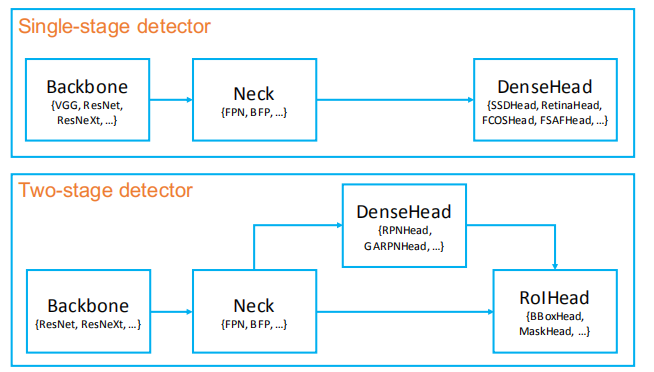
\includegraphics[width=5cm, height=3cm]{./pic/mmdetect.png}
 	\caption{ Framework }
 	\end{minipage}
 	\begin{minipage}[t]{0.48\textwidth}
 	\centering
	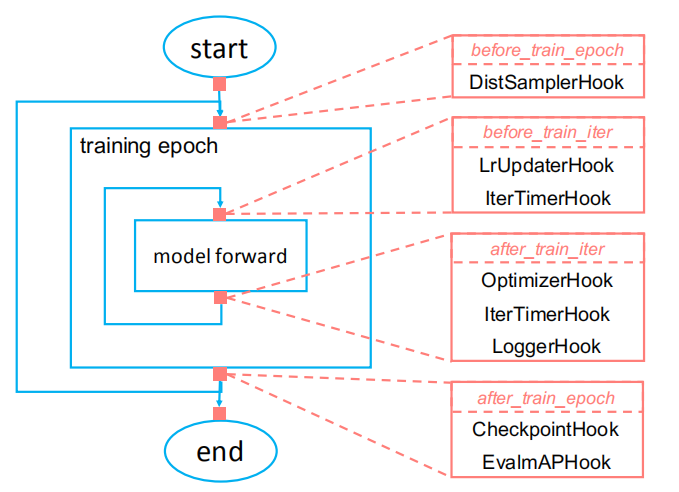
\includegraphics[width=5cm,height=3cm]{./pic/mmdetect_pipe.png}
	\caption{Trainning pipeline}
	\label{trainpipe_pic}
 	\end{minipage}
 \end{figure}

 % \newpage
 \subsection{总体逻辑}
从tools/train.py中能看到整体可分如下4个步骤:\\
1. mmcv.Config.fromfile从配置文件解析配置信息,并做适当更新,包括环境搜集,预加载模型文件,分布式设置,日志记录等
 
 \noindent 2. mmdet.models中的build\_detector根据配置信息构造模型
 \begin{adjustwidth}{0.5cm}{0cm}
 2.1 build系列函数调用build\_from\_cfg函数,按type关键字从注册表中获取相应的
 对象,对象的具名参数在注册文件中赋值。\\
2.2 registr.py放置了模型的组件注册器。其中注册器的register\_module成员函数是一
 个装饰器功能函数,在具体的类对象$A$头上装饰@X.register
 \_module,并同时在$A$对象所在包的初始化文件中调用$A$,即可将$A$保存
 到registry.module\_dict中,完成注册。\\
 2.3 目前包含BACKBONES,NECKS,ROI\_EXTRACTORS,SHARED\_
 HEADS,HEADS,LOSSES,DETECTORS七个模型相关注册器,另外还有数据类,优化器等注册器。\\
 \end{adjustwidth}
 
\noindent 3. build\_dataset根据配置信息获取数据类
\begin{adjustwidth}{0.5cm}{0cm} 
 3.1 coco,cityscapes,voc,wider\_face等数据(数据类扩展见后续例子)。\\
\end{adjustwidth}
 
 \noindent 4.train\_detector模型训练流程
 \begin{adjustwidth}{0.5cm}{0cm} 
 4.1 数据loader化,模型分布式化,优化器选取\\
 4.2 进入runner训练流程(来自mmcv库,采用hook方式,整合了pytorch训练流程)\\
4.2 训练pipelines可见\ref{trainpipe_pic},具体细节见后续展开。\\
\end{adjustwidth}

\noindent 后续说说配置文件,注册机制和训练逻辑。


\section{配置,注册}
\subsection{配置类}
配置方式支持python/json/yaml,从mmcv的Config解析,其功能同maskrcnn-benchmark的yacs类似,将字典的取值方式属性化.这里帖部分代码,以供学习。

\lstset{style=mystyle}
\begin{lstlisting}[language=Python]
class Config(object):
    ...
    @staticmethod
    def _file2dict(filename):
        filename = osp.abspath(osp.expanduser(filename))
        check_file_exist(filename)
        if filename.endswith('.py'):
            with tempfile.TemporaryDirectory() as temp_config_dir:
                shutil.copyfile(filename,
                                osp.join(temp_config_dir, '_tempconfig.py'))
                sys.path.insert(0, temp_config_dir)
                mod = import_module('_tempconfig')
                sys.path.pop(0)
                cfg_dict = {
                    name: value
                    for name, value in mod.__dict__.items()
                    if not name.startswith('__')
                }
                # delete imported module
                del sys.modules['_tempconfig']
        elif filename.endswith(('.yml', '.yaml', '.json')):
            import mmcv
            cfg_dict = mmcv.load(filename)
        else:
            raise IOError('Only py/yml/yaml/json type are supported now!')

        cfg_text = filename + '\n'
        with open(filename, 'r') as f:
            cfg_text += f.read()
        # 2.0新增的配置文件的组合继承
        if '_base_' in cfg_dict:
            cfg_dir = osp.dirname(filename)
            base_filename = cfg_dict.pop('_base_')
            base_filename = base_filename if isinstance(
                base_filename, list) else [base_filename]

            cfg_dict_list = list()
            cfg_text_list = list()
            for f in base_filename:
                # 递归,可搜索staticmethod and recursion
                # 静态方法调静态方法,类方法调静态方法
                _cfg_dict, _cfg_text = Config._file2dict(osp.join(cfg_dir, f))
                cfg_dict_list.append(_cfg_dict)
                cfg_text_list.append(_cfg_text)

            base_cfg_dict = dict()
            for c in cfg_dict_list:
                if len(base_cfg_dict.keys() & c.keys()) > 0:
                    raise KeyError('Duplicate key is not allowed among bases')
                base_cfg_dict.update(c)
            # 合并
            Config._merge_a_into_b(cfg_dict, base_cfg_dict)
            cfg_dict = base_cfg_dict

            # merge cfg_text
            cfg_text_list.append(cfg_text)
            cfg_text = '\n'.join(cfg_text_list)

        return cfg_dict, cfg_text
    
    ...
    # 获取key值
    def __getattr__(self, name):
        return getattr(self._cfg_dict, name)
    # 序列化
    def __getitem__(self, name):
        return self._cfg_dict.__getitem__(name)
    # 将字典属性化主要用了__setattr__
    def __setattr__(self, name, value):
        if isinstance(value, dict):
            value = ConfigDict(value)
        self._cfg_dict.__setattr__(name, value)
    # 更新key值
    def __setitem__(self, name, value):
        if isinstance(value, dict):
            value = ConfigDict(value)
        self._cfg_dict.__setitem__(name, value)
    # 迭代器
    def __iter__(self):
        return iter(self._cfg_dict)
        
\end{lstlisting}

主要考虑点是自己怎么实现类似的东西,核心点就是python的基本魔法函数的应用,可同时参考yacs。

\subsection{注册器}
把基本对象放到一个继承了字典的对象中,实现了对象的灵活管理。
\lstset{style=mystyle}
\begin{lstlisting}[language=Python]
import inspect
from functools import partial
import mmcv

class Registry(object):
    # 2.0 放到mmcv中

    def __init__(self, name):
        self._name = name
        self._module_dict = dict()
    @property
    def name(self):
        return self._name
    @property
    def module_dict(self):
        return self._module_dict

    def get(self, key):
        return self._module_dict.get(key, None)

    def _register_module(self, module_class, force=False):
        """Register a module.

        Args:
            module (:obj:`nn.Module`): Module to be registered.
        """
        if not inspect.isclass(module_class):
            raise TypeError('module must be a class, but got {}'.format(
                type(module_class)))
        module_name = module_class.__name__
        if not force and module_name in self._module_dict:
            raise KeyError('{} is already registered in {}'.format(
                module_name, self.name))
        self._module_dict[module_name] = module_class   # 类名:类

    def register_module(self, cls=None, force=False):
        # 作为类cls的装饰器
        if cls is None:
            # partial函数(类)固定参数,返回新对象,递归不是很清楚
            return partial(self.register_module, force=force)    
        self._register_module(cls, force=force)   # 将cls装进当前Registry对象的中_module_dict
        return cls    # 返回类

def build_from_cfg(cfg, registry, default_args=None):
	assert isinstance(cfg, dict) and 'type' in cfg
	assert isinstance(default_args, dict) or default_args is None
	args = cfg.copy()
	obj_type = args.pop('type')
	if mmcv.is_str(obj_type):
		# 从注册类中拿出obj_type类
		obj_cls = registry.get(obj_type)
		if obj_cls is None:
			raise KeyError('{} is not in the {} registry'.format(
				obj_type, registry.name))
	elif inspect.isclass(obj_type):
		obj_cls = obj_type
	else:
		raise TypeError('type must be a str or valid type, but got {}'.format(
			type(obj_type)))
	if default_args is not None:
		# 增加一些新的参数
		for name, value in default_args.items():
			args.setdefault(name, value)
	return obj_cls(**args)    # **args是将字典解析成位置参数(k=v)。
\end{lstlisting}


\section{数据处理}
\label{sec:detail}
数据处理可能是炼丹师接触最为密集的了,因为通常情况,除了数据的离线处理,写个数据类,就可以炼丹了。但本节主要涉及数据的在线处理,更进一步应该是检测分割数据的pytorch处理方式。虽然mmdet将常用的数据都实现了,而且也实现了中间通用数据格式,但,这和模型,损失函数,性能评估的实现也相关,比如你想把官网的centernet完整的改成mmdet风格,就能看到(看起来没必要)。

\subsection{检测分割数据}
看看配置文件,数据相关的有data dict,里面包含了train,val,test的路径信息,用于数据类初始化,有pipeline,将各个函数及对应参数以字典形式放到列表里,是对pytorch原装的transforms+compose,在检测,分割相关数据上的一次封装,使得形式更加统一。

从builder.py中build\_dataset函数能看到,构建数据有三种方式,ConcatDataset,RepeatDataset和从注册器中提取。其中dataset\_wrappers.py中ConcatDataset和RepeatDataset意义自明,前者继承自pytorch原始的ConcatDataset,
将多个数据集整合到一起,具体为把不同序列(可参考\href{https://docs.python.org/zh-cn/3/library/collections.abc.html}
{容器的抽象基类})的长度相加,\_\_getitem\_\_函数对应index替换一下。
后者就是单个数据类(序列)的多次重复。就功能来说,前者提高数据丰富度,后者可解决数据太少使得loading时间长的问题(见代码注释)。
而被注册的数据类在datasets下一些熟知的数据名文件中。其中,基类为custom.py中的CustomDataset,coco继承自它,
cityscapes继承自coco,xml\_style的XMLDataset继承CustomDataset,然后wider\_face,voc均继承自XMLDataset。因此这里先分析一下CustomDataset。

CustomDataset 记录数据路径等信息,解析标注文件,将每一张图的所有信息以字典作为数据结构存在results中,然后进入pipeline:数据增强相关操作,代码如下:

\lstset{style=mystyle}
\begin{lstlisting}[language=Python]
	self.pipeline = Compose(pipeline)   
	# Compose是实现了__call__方法的类,其作用是使实例能够像函数一样被调用,同时不影响实例本身的生命周期
def pre_pipeline(self, results):
	# 扩展字典信息
	results['img_prefix'] = self.img_prefix
	results['seg_prefix'] = self.seg_prefix
	results['proposal_file'] = self.proposal_file
	results['bbox_fields'] = []
	results['mask_fields'] = []
	results['seg_fields'] = []

def prepare_train_img(self, idx):
	img_info = self.img_infos[idx]
	ann_info = self.get_ann_info(idx)
	# 基本信息,初始化字典
	results = dict(img_info=img_info, ann_info=ann_info)
	if self.proposals is not None:
		results['proposals'] = self.proposals[idx]
	self.pre_pipeline(results)
	return self.pipeline(results)    # 数据增强

def __getitem__(self, idx):
	if self.test_mode:
		return self.prepare_test_img(idx)
	while True:
		data = self.prepare_train_img(idx)
		if data is None:
			idx = self._rand_another(idx)
			continue
		return data
\end{lstlisting}

这里数据结构的选取需要注意一下,字典结构,在数据增强库albu中也是如此处理,因此可以快速替换为albu中的算法。另外每个数据类增加了各自的evaluate函数。evaluate基础函数在mmdet.core.evaluation中,后做补充。

mmdet的数据处理,\textbf{字典结构},\textbf{pipeline},\textbf{evaluate}是三个关键部分。其他所有类的文件解析部分,数据筛选等,看看即可。因为我们知道,pytorch读取数据,是将序列转化为迭代器后进行io操作,所以在dataset下除了pipelines外还有loader文件夹,里面实现了分组,分布式分组采样方法,以及调用了mmcv中的collate函数(此处为1.x版本,2.0版本将loader移植到了builder.py中),且build\_dataloader封装的DataLoader最后在
train\_detector中被调用,这部分将在后面补充,这里说说pipelines。

返回maskrcnn的配置文件(1.x,2.0看base config),可以看到训练和测试的不同之处:LoadAnnotations,MultiScaleFlipAug,DefaultFormatBundle和Collect。
额外提示,虽然测试没有LoadAnnotations,根据CustomDataset可知,它仍需标注文件,这和inference的pipeline不同,也即这里的test实为evaluate。

\lstset{style=mystyle}
\begin{lstlisting}[language=Python]
# 序列中的dict可以随意删减,增加,属于数据增强调参内容
train_pipeline = [
    dict(type='LoadImageFromFile'),
    dict(type='LoadAnnotations', with_bbox=True, with_mask=True),
    dict(type='Resize', img_scale=(1333, 800), keep_ratio=True),
    dict(type='RandomFlip', flip_ratio=0.5),
    dict(type='Normalize', **img_norm_cfg),
    dict(type='Pad', size_divisor=32),
    dict(type='DefaultFormatBundle'),
    dict(type='Collect', keys=['img', 'gt_bboxes', 'gt_labels', 'gt_masks']),
]

test_pipeline = [
    dict(type='LoadImageFromFile'),
    dict(
        type='MultiScaleFlipAug',
        img_scale=(1333, 800),
        flip=False,
        transforms=[
            dict(type='Resize', keep_ratio=True),
            dict(type='RandomFlip'),
            dict(type='Normalize', **img_norm_cfg),
            dict(type='Pad', size_divisor=32),
            dict(type='ImageToTensor', keys=['img']),
            dict(type='Collect', keys=['img']),
        ])
]
\end{lstlisting}
最后这些所有操作被Compose串联起来,代码如下:

\lstset{style=mystyle}
\begin{lstlisting}[language=Python]
@PIPELINES.register_module
class Compose(object):

	def __init__(self, transforms):
		assert isinstance(transforms, collections.abc.Sequence)  # 列表是序列结构
		self.transforms = []
		for transform in transforms:
			if isinstance(transform, dict):
				transform = build_from_cfg(transform, PIPELINES)
				self.transforms.append(transform)
			elif callable(transform):
				self.transforms.append(transform)
			else:
				raise TypeError('transform must be callable or a dict')

	def __call__(self, data):
		for t in self.transforms:
			data = t(data)
			if data is None:
				return None
		return data
\end{lstlisting}
上面代码能看到,配置文件中pipeline中的字典传入build\_from\_cfg函数,逐一实现了各个增强类(方法)。
扩展的增强类均需实现\_\_call\_\_方法,这和pytorch原始方法是一致的。


有了以上认识,重新梳理一下pipelines的逻辑,由三部分组成,load,transforms,和format。
load相关的LoadImageFromFile,LoadAnnotations都是字典results进去,字典results出来。具体代码看下便知,
LoadImageFromFile增加了'filename','img','img\_shape','ori\_shape','pad\_shape',
'scale\_factor','img\_norm\_cfg'字段。其中img是numpy格式。LoadAnnotations从results['ann\_info']中解析出bboxs,masks,labels等信
息。注意coco格式的原始解析来自pycocotools,包括其评估方法,这里关键是字典结构(这个和模型损失函数,评估等相关,统一结构,使得代码统一)。
transforms中的类作用于字典的values,也即数据增强。format中的DefaultFormatBundle是将数据转成mmcv扩展的容器类格式DataContainer。
另外Collect会根据不同任务的不同配置,从results中选取只含keys的信息生成新的字典,具体看下该类帮助文档。
这里看一下从numpy转成tensor的代码:

\lstset{style=mystyle}
\begin{lstlisting}[language=Python]
def to_tensor(data):
    """Convert objects of various python types to :obj:`torch.Tensor`.

    Supported types are: :class:`numpy.ndarray`, :class:`torch.Tensor`,
    :class:`Sequence`, :class:`int` and :class:`float`.
    """
    if isinstance(data, torch.Tensor):
        return data
    elif isinstance(data, np.ndarray):
        return torch.from_numpy(data)
    elif isinstance(data, Sequence) and not mmcv.is_str(data):
        return torch.tensor(data)
    elif isinstance(data, int):
        return torch.LongTensor([data])
    elif isinstance(data, float):
        return torch.FloatTensor([data])
    else:
        raise TypeError('type {} cannot be converted to tensor.'.format(
			type(data)))
	以上代码告诉我们,基本数据类型,需掌握。
\end{lstlisting}

那么DataContainer是什么呢?它是对tensor的封装,将results中的tensor转成DataContainer格式,实际上只是增加了几个property函数,
cpu\_only,stack,padding\_value,pad\_dims,其含义自明,以及size,dim用来获取数据的维度,形状信息。
考虑到序列数据在进入DataLoader时,需要以batch方式进入模型,那么通常的collate\_fn会要求tensor数据的形状一致。但是这样不是很方便,
于是有了DataContainer。它可以做到载入GPU的数据可以保持统一shape,并被stack,也可以不stack,也可以保持原样,或者在非batch维度上做pad。
当然这个也要对default\_collate进行改造,mmcv在parallel.collate中实现了这个。

collate\_fn是DataLoader中将序列dataset组织成batch大小的函数,这里帖三个普通例子:

\lstset{style=mystyle}
\begin{lstlisting}[language=Python]
def collate_fn_1(batch):
	# 这是默认的,明显batch中包含相同形状的img\_tensor和label
	return tuple(zip(*batch))
	
def coco_collate_2(batch):
	# 传入的batch数据是被albu增强后的(字典结构)
    imgs = [s['image'] for s in batch]    # tensor, h, w, c->c, h, w , handle at transform in __getitem__
    annots = [s['bboxes'] for s in batch]
    labels = [s['category_id'] for s in batch]

	# 以当前batch中图片annot数量的最大值作为标记数据的第二维度值,空出的就补-1。
    max_num_annots = max(len(annot) for annot in annots)
    annot_padded = np.ones((len(annots), max_num_annots, 5))*-1

    if max_num_annots > 0:
        for idx, (annot, lab) in enumerate(zip(annots, labels)):
            if len(annot) > 0:
                annot_padded[idx, :len(annot), :4] = annot
				# 不同模型,损失值计算可能不同,这里ssd结构需要改为xyxy格式并且要做尺度归一化
				# 这一步完全可以放到\_\_getitem\_\_中去,只是albu的格式需求问题。
                annot_padded[idx, :len(annot), 2] += annot_padded[idx, :len(annot), 0]    #  xywh-->x1,y1,x2,y2 for general box,ssd target assigner
                annot_padded[idx, :len(annot), 3] += annot_padded[idx, :len(annot), 1]    # contains padded -1 label
                annot_padded[idx, :len(annot), :] /=  640    # priorbox for ssd primary target assinger
                annot_padded[idx, :len(annot), 4] = lab
	return torch.stack(imgs, 0), torch.FloatTensor(annot_padded)
	
def detection_collate_3(batch):
    targets = []
    imgs = []
    for _, sample in enumerate(batch):
        for _, img_anno in enumerate(sample):
            if torch.is_tensor(img_anno):
                imgs.append(img_anno)
            elif isinstance(img_anno, np.ndarray):
                annos = torch.from_numpy(img_anno).float()
                targets.append(annos)
    return torch.stack(imgs, 0), targets    # 做了stack, DataContainer可以不做stack
\end{lstlisting}

以上就是数据处理的相关内容。
最后再用DataLoader封装拆成迭代器,其相关细节,sampler等暂略。
\lstset{style=mystyle}
\begin{lstlisting}[language=Python]
data_loader = DataLoader(
	dataset,
	batch_size=batch_size,
	sampler=sampler,
	num_workers=num_workers,
	collate_fn=partial(collate, samples_per_gpu=imgs_per_gpu),
	pin_memory=False,
	worker_init_fn=init_fn,
	**kwargs)
\end{lstlisting}


\section{训练流程}
训练流程的包装过程大致如下:tools/train.py->apis/train.py->mmcv/
runner.py->mmcv/hook.py(后面是分散的),其中runner维护了数据信息,优化器,
日志系统,训练loop中的各节点信息,模型保存,学习率等.另外补充一点,以上包装过程,
在mmdet中无处不在,包括mmcv的代码也是对日常频繁使用的函数进行了统一封装.

\label{trainpipeline}
\subsection{训练逻辑}
图见\ref{trainpipe_pic},注意它的四个层级.代码上,主要查看apis/train.py, mmcv中的runner相关文件.核心围绕Runner,Hook两个类.
Runner将模型,批处理函数batch\_pro
cessor,优化器作为基本属性,训练过程中与训练状态,各节点相关的信息
被记录在mode,\_hooks,\_epoch,\_iter,\_inner\_iter,\_max\_epochs,
\_max\_iters中,这些信息维护了训练过程中插入不同hook的操作方式.
理清训练流程只需看Runner的成员函数run.在run里会根据mode按配置中workflow的epoch循环调用train和val函数,跑完所有的epoch.比如train:
\lstset{style=mystyle}
\begin{lstlisting}[language=Python]
 def train(self, data_loader, **kwargs):
	self.model.train()
	self.mode = 'train'    # 改变模式
	self.data_loader = data_loader
	self._max_iters = self._max_epochs * len(data_loader)    # 最大batch循环次数
	self.call_hook('before_train_epoch')    # 根据名字获取hook对象函数
	for i, data_batch in enumerate(data_loader):
		self._inner_iter = i    # 记录训练迭代轮数
		self.call_hook('before_train_iter')    # 一个batch前向开始
		outputs = self.batch_processor(
			self.model, data_batch, train_mode=True, **kwargs)
		self.outputs = outputs
		self.call_hook('after_train_iter')    # 一个batch前向结束
		self._iter += 1    # 方便resume时,知道从哪一轮开始优化

	self.call_hook('after_train_epoch')    # 一个epoch结束
	self._epoch += 1    # 记录训练epoch状态,方便resume

\end{lstlisting}

上面需要说明的是自定义hook类,自定义hook类需继承mmcv的Hook类,其默认了6+8+4个成员函数,也即\ref{trainpipe_pic}所示的6个层级节点,外加2*4个区分train和val的节点记录函数,以及4个边界检查函数.从train.py中容易看出,在训练之前,已经将需要的hook函数注册到Runner的self.\_hook中了,包括从配置文件解析的优化器,学习率调整函数,模型保存,一个batch的时间记录等(注册hook算子在self.\_hook中按优先级升序排列).这里的call\_hook函数定义如下:
\lstset{style=mystyle}
\begin{lstlisting}[language=Python]
def call_hook(self, fn_name):
	for hook in self._hooks:
		getattr(hook, fn_name)(self)
\end{lstlisting}

容易看出,在训练的不同节点,将从注册列表中调用实现了该节点函数的类成员函数.比如

\lstset{style=mystyle}
\begin{lstlisting}[language=Python]
class OptimizerHook(Hook):

    def __init__(self, grad_clip=None):
        self.grad_clip = grad_clip

    def clip_grads(self, params):
        clip_grad.clip_grad_norm_(
            filter(lambda p: p.requires_grad, params), **self.grad_clip)

    def after_train_iter(self, runner):
        runner.optimizer.zero_grad()
        runner.outputs['loss'].backward()
        if self.grad_clip is not None:
            self.clip_grads(runner.model.parameters())
        runner.optimizer.step()
\end{lstlisting}
将在每个train\_iter后实现反向传播和参数更新.

学习率优化相对复杂一点,其基类LrUpdaterHook,实现了before\_run, before\_train\_epoch, before\_train\_iter三个hook函数,意义自明.
这里选一个余弦式变化,稍作说明:

\lstset{style=mystyle}
\begin{lstlisting}[language=Python]
class CosineLrUpdaterHook(LrUpdaterHook):

    def __init__(self, target_lr=0, **kwargs):
        self.target_lr = target_lr
        super(CosineLrUpdaterHook, self).__init__(**kwargs)

    def get_lr(self, runner, base_lr):
        if self.by_epoch:
            progress = runner.epoch
            max_progress = runner.max_epochs
        else:
            progress = runner.iter    # runner需要管理各节点信息的原因之一
            max_progress = runner.max_iters
        return self.target_lr + 0.5 * (base_lr - self.target_lr) * \
			(1 + cos(pi * (progress / max_progress)))
\end{lstlisting}
从get\_lr可以看到,学习率变换周期有两种,epoch->max\_epoch,或者更大的iter->max\_iter,
后者表明一个epoch内不同batch的学习率可以不同,因为没有什么理论,所有这两种方式都行.
其中base\_lr为初始学习率,target\_lr为学习率衰减的上界,而当前学习率即为返回值.



\section{Core}

\subsection{anchor}
\label{core:anchor}
anchor首先来源于rcnn,在我看来,anchor利用强监督的特点,在原图上构造了完整的bbox空间(非数学意义的空间),然后根据人为标定bbox,选出有效的拟合集合(子空间,非严格表达),从而使得优化变得更有效(原本是实现了end2end)。

AnchorGenerator类为不同特征层生成anchor,其中特征层上单个像素的anchor是以此像素为中心,
按给定的尺度和扩展比率生成,也即一个像素对应的anchor数为len(scales)*len(ratios)。

输入参数base\_size, scales, ratios一般作用于非retinta类网络,含义分别表示:anchor在特征层上的基础大小(特征层相对于原图的stride),anchor在特征层上的尺度大小(可以多个,增加感受野),anchor在保持基础大小不变的情况下的长宽比.
比如输入图像大小(640*640), 选择(p2, p3)作为其特征层,则p2大小为(160*160),base\_ size=4,若设定ratios=[0.5,1.0,2.0], scales=[8, 16],
则在p2上一格对应的base\_anchor的(w,h)为[(45.25,22.63),  (90.51, 45.25),
 (32.00, 32.00),  (64.00, 64.00), (22.63, 45.25),(45.25, 90.51)].其中$64=4*16*1,90.51=4*16*\sqrt{2}, 22.63=4*8/\sqrt{2}.$
 那么每一格所对应的6个base\_anchor相对于中心点的偏移量即为(v2.0不取整):
\lstset{style=mystyle}
\begin{lstlisting}[language=Python]
	
											[[-21.,  -9.,  24.,  12.],
											[-43., -21.,  46.,  24.],
											[-14., -14.,  17.,  17.],
											[-30., -30.,  33.,  33.],
											[ -9., -21.,  12.,  24.],
											[-21., -43.,  24.,  46.]]

\end{lstlisting}

而retina等网络会存在octave\_base\_scale,scales\_per\_octave,其含义和上面保持对应。

因为此处得到的anchor是以特征图为坐标系的,所以要得到原图上的anchor,还得把中心点变为对应到原图的上的点。
那么回到源代码,容易看出,gen\_single\_level\_base\_anchors得到单个特征层的所有anchor,gen\_base\_anchors将
不同特征层的anchor汇集到列表里,single\_level\_grid
\_anchors将单个特征层的anchor变为原图中,grid\_anchors则将
所有特征汇集到列表中,列表每个元素为一个tensor,记录了对应特征层上的所有anchor坐标。
代码涉及到两个技巧:
\lstset{style=mystyle}
\begin{lstlisting}[language=Python]
# 1.gen_single_level_base_anchors
ws = (w * w_ratios[:, None] * self.scales[None, :]).view(-1)    # shape: (len(ratios), len(scales))
hs = (h * h_ratios[:, None] * self.scales[None, :]).view(-1)

# 2.single_level_grid_anchors
shifts = torch.stack([shift_xx, shift_yy, shift_xx, shift_yy], dim=-1)
shifts = shifts.type_as(base_anchors)
# first feat_w elements correspond to the first row of shifts
# add A anchors (1, A, 4) to K shifts (K, 1, 4) to get
# shifted anchors (K, A, 4), reshape to (K*A, 4)
# base_anchors:(fw*hw*num_anchors, 4), shifts:(fw*hw, 4)
all_anchors = base_anchors[None, :, :] + shifts[:, None, :]    #此处直接理解较难
all_anchors = all_anchors.view(-1, 4)
\end{lstlisting}


另一个PointGenerator代码如下:
\lstset{style=mystyle}
\begin{lstlisting}[language=Python]
class PointGenerator(object):
	def _meshgrid(self, x, y, row_major=True):
		xx = x.repeat(len(y))
		yy = y.view(-1, 1).repeat(1, len(x)).view(-1)
		if row_major:
			return xx, yy   # (xx[i],yy[j])为一个矩阵A_xy的坐标(i,j), dim(xx)=1时
		else:
			return yy, xx

	def grid_points(self, featmap_size, stride=16, device='cuda'):
		feat_h, feat_w = featmap_size
		shift_x = torch.arange(0., feat_w, device=device) * stride    # 特征网格对应到原图网格
		shift_y = torch.arange(0., feat_h, device=device) * stride
		shift_xx, shift_yy = self._meshgrid(shift_x, shift_y)
		stride = shift_x.new_full((shift_xx.shape[0], ), stride)
		shifts = torch.stack([shift_xx, shift_yy, stride], dim=-1)  # x, y和对应点的stride大小
		all_points = shifts.to(device)
		return all_points
\end{lstlisting}

代码上,主要的难点在于高维张量的处理。

\subsection{bbox}

\subsubsection{coder}
bbox的编码是基础重要的,一家之言:anchor genertor让优化空间合理,bbox编码让优化更合理(guided anchor处在这两者之间)。
通常bbox连归一化都不做的,效果不会好到哪里去(可以试试retinaface)。但是在不同方法体系里面,就不好说了,比如以中心点
表示方式的CenterNet,对$w, h$做回归,就没有编码,直接拟合$\Delta w, \Delta h$,但它是在下采样$1/4$后的特征图上,
也即尺度上还是除了4。总归而言,要让优化对象存在一个合理的空间上,才是本质的。

one, two stage的bbox编码方式,来源于14年Ross Girshick等人写的rcnn,
其编码为
$$
\begin{aligned}
	t_{x} &=\left(G_{x}-P_{x}\right) / P_{w} \label{1} \\
	t_{y} &=\left(G_{y}-P_{y}\right) / P_{h} \label{2}\\
	t_{w} &=\log \left(G_{w} / P_{w}\right)  \label{3}\\
	t_{h} &=\log \left(G_{h} / P_{h}\right)  \label{4}
\end{aligned}
$$
此处$P$是anchor,$G$是标框。

解码为:
$$
\begin{aligned}
	\hat{G}_{x} &=P_{w} d_{x}(P)+P_{x} \\
	\hat{G}_{y} &=P_{h} d_{y}(P)+P_{y} \\
	\hat{G}_{w} &=P_{w} \exp \left(d_{w}(P)\right) \\
	\hat{G}_{h} &=P_{h} \exp \left(d_{h}(P)\right)
\end{aligned}
$$
% 相应的优化函数我也帖一下:
% $$
% \mathbf{w}_{\star}=\underset{\hat{\mathbf{w}}_{\star}}{\operatorname{argmin}}
%  \sum_{i}^{N}\left(t_{\star}^{i}-\hat{\mathbf{w}}_{\star}^{\mathrm{T}}
%  \phi_{5}\left(P^{i}\right)\right)^{2}+\lambda\left\|\hat{\mathbf{w}}_{\star}\right\|^{2}
% $$
% 关于这种编码的合理性,见\ref{sub:anchorhead}的分析。

那么代码如何实现呢?

\lstset{style=mystyle}
\begin{lstlisting}[language=Python]
class BaseBBoxCoder(metaclass=ABCMeta):

	def __init__(self, **kwargs):
		pass
	@abstractmethod
	def encode(self, bboxes, gt_bboxes):
		pass
	@abstractmethod
	def decode(self, bboxes, bboxes_pred):
		pass

def bbox2delta(proposals, gt, means=(0., 0., 0., 0.), stds=(1., 1., 1., 1.)):
	assert proposals.size() == gt.size()

	proposals = proposals.float()    # 浮点数
	gt = gt.float()
	px = (proposals[..., 0] + proposals[..., 2]) * 0.5    # 中心点(x1+x2)/2
	py = (proposals[..., 1] + proposals[..., 3]) * 0.5 
	pw = proposals[..., 2] - proposals[..., 0]    
	ph = proposals[..., 3] - proposals[..., 1]

	gx = (gt[..., 0] + gt[..., 2]) * 0.5    
	gy = (gt[..., 1] + gt[..., 3]) * 0.5
	gw = gt[..., 2] - gt[..., 0]    # 宽(x2 - x1) = w
	gh = gt[..., 3] - gt[..., 1]

	dx = (gx - px) / pw    # \eqref{1}
	dy = (gy - py) / ph    # \eqref{2}
	dw = torch.log(gw / pw)
	dh = torch.log(gh / ph)    # \eqref{4}
	deltas = torch.stack([dx, dy, dw, dh], dim=-1)    # 最后一维度stack

	means = deltas.new_tensor(means).unsqueeze(0)    # new_tensor和unsqueeze(扩张维度)
	stds = deltas.new_tensor(stds).unsqueeze(0)
	deltas = deltas.sub_(means).div_(stds)    # sub_ 和 sub 的区别

	return deltas

gx = torch.addcmul(px, 1, pw, dx)  # gx = px + pw * dx
gy = torch.addcmul(py, 1, ph, dy)  # gy = py + ph * dy

# torch.addcmul(input, tensor1, tensor2, *, value=1, out=None) → Tensor
# outi​=input_i​+value×tensor_1i​×tensor_2i​
\end{lstlisting}

stack, new\_tensor, unsqueeze, div\_可以学习一下。另外为何$\Delta$坐标系(说法不严谨,
但可以理解,cv论文经常这样)要做高斯归一化变换呢?可参考\href{https://arxiv.org/abs/1904.04620}{Gaussian YOLOv3}。
我的理解,将优化空间映射到高斯$\mu-\sigma$分布中。

在解码函数delta2bbox有如下函数需要注意一下(tensor.*):
repeat, clamp, expand\_as, exp, torch.addcmul, view\_as。

另外一种编码方式,来自19年Chenchen Zhu等人写的\href{https://arxiv.org/abs/1903.00621}{FSAF}。
将(x1, y1,x2, y2)编码为(top, bottom, left, right),含义自明。代码上需要注意的是$w, h$的归一化以及整体
的归一化因子,默认除以4。此编码对应的bbox loss 也将变为Iou 系列 Loss, 若说明,也应该是在模型解析部分补充。

\subsubsection{assigners}
assign主要给特征图上的anchor赋予有意义的监督信息,从而使优化更为有效。那么自然他的参数至少包含
anchors,gt\_bboxes,gt\_labels。实际因为数据的复杂,或许有gt\_bboxes\_ignore等信息。
assign的机制可总结为如下四点:
\begin{itemize}
    \item[1.] 将所有框置为背景(label置-1)
    \item[2.] 将与所有gts的iou小于neg\_iou\_thr的置为0
    \item[3.] 将与所有gt的max(iou)大于pos\_iou\_thr的框置为对应gt
    \item[4.] 对每个gt,将与其iou最大的框置为gt
\end{itemize}
关于上述四点:用生成的bbox去拟合实际的bbox,那么实际的bbox至少有一个可以优化的对象。

有了这些认识,代码就相对容易了。
\lstset{style=mystyle}
\begin{lstlisting}[language=Python]
@BBOX_ASSIGNERS.register_module()
class MaxIoUAssigner(BaseAssigner):
    # 关键代码(BaseAssigner,抽象基类)
    # assign:
    ...   # gt太多,就cpu上计算
    overlaps = self.iou_calculator(gt_bboxes, bboxes)  # gt在前,更快吧
    ...
    # assign_wrt_overlaps
    # 1. 默认全部为背景-1
    assigned_gt_inds = overlaps.new_full((num_bboxes, ),
                                         -1,
                                         dtype=torch.long)
    # 每个bbox与所有gt的最大iou值和index
    max_overlaps, argmax_overlaps = overlaps.max(dim=0)
    # 每个gt与所有bbox的最大iou值和index 
    gt_max_overlaps, gt_argmax_overlaps = overlaps.max(dim=1)
    # 2 负样本置0
    assigned_gt_inds[(max_overlaps >= 0)
                             & (max_overlaps < self.neg_iou_thr)] = 0
    # 3 argmax_overlaps的值gt的维度上的index,但其本身的维度是bbox的维度
    pos_inds = max_overlaps >= self.pos_iou_thr
    assigned_gt_inds[pos_inds] = argmax_overlaps[pos_inds] + 1
    
    # 4 bbox和gt的max(iou)对应的gt未必是此bbox的最好设定,得从gt的max(iou)为出发点,会更好。
    if self.match_low_quality:
            for i in range(num_gts):
                if gt_max_overlaps[i] >= self.min_pos_iou:
                    if self.gt_max_assign_all:
                        max_iou_inds = overlaps[i, :] == gt_max_overlaps[i]
                        assigned_gt_inds[max_iou_inds] = i + 1
                    else:
                        assigned_gt_inds[gt_argmax_overlaps[i]] = i + 1
    # 最终结果被AssignResult(num_gts, assigned_gt_inds, max_overlaps, labels=assigned_labels)
    # 包装,方便调试,查看算法的数据状态
\end{lstlisting}

\subsubsection{sampler}
sample主要为two-stage服务.已实现的有RandomSampler,CombinedSampler,OHEMSampler,InstanceBalancedPosSampler,IoUBalancedNegSampler,这些均继承自抽象类BaseSampler,继承自它的的类必须完成\_sample\_pos,
\_sample\_neg两函数.按照python的语法,子类可以使用raise NotImplementedError来避免不能实例化的问题,PseudoSampler即是如此,它重写了sample函数,该函数并没有做任何筛选。RandomSampler可算中间类,意思自明。
另外,采样只是在做bbox的index选取,并不会改变bbox等的形状,这在最后算损失函数时,只需要乘以选取的mask即可。

\subsubsection{iou\_calculators}
torch版本的iou计算,主要注意点是张量计算,广播机制。

\lstset{style=mystyle}
\begin{lstlisting}[language=Python]
# bboxes1 (Tensor): shape (m, 4) in <x1, y1, x2, y2> format or empty.
# bboxes2 (Tensor): shape (n, 4) in <x1, y1, x2, y2> format or empty.
lt = torch.max(bboxes1[:, None, :2], bboxes2[:, :2])  # 这里m!=n, [m, None, 2] + [n, 2] --> [m, n, 2] 
# None 技巧
\end{lstlisting}

\subsection{evaluate}
mAP的含义可以参考\href{https://zhuanlan.zhihu.com/p/55575423}{mmAP浅析一}
我就不滥竽充数了,将其部分摘录于此:

"
我们都知道,评价一个图像分类结果的性能,只需要看预测类别是否正确即可,在一个数据集上面,我们可以很容易地得出一个平均准确率。可是目标检测的输出目标数量和真实目标数量都是不固定的(前文提到的非结构化的特性),因此评判时要考虑的就不仅是“对错”这么简单了,我们需要考虑的有:如果漏掉了一个目标对性能有多大损伤?如果多检测出了一个目标对性能有多大损伤?如果检测出来的位置信息有所偏差对性能有多大损伤?进一步地,在这么多的检测结果中,总有一些是检测器十分笃定的,有一些是模棱两可的。如果检测器对多检测出来的那个目标本身也不太确定呢?如果检测器最满意最信任的那个检测结果出错了呢?换言之:一个检测结果对性能的影响,是否应该和检测器对它的满意程度(置信度)相关?以及,检测错了一个稀有的物体和检测错了一个常见的物体所带来的性能损伤是否应该相同?......

刚刚提到的所有问题,mmAP都要一一给出答案。

首先是位置偏差问题。有的使用场景对位置的准确度要求不高,有的则要求精确定位。因此,mmAP先按位置准确度的需求进行划分,设置一组IOU阈值,这组阈值为 (0.5, 0.55, 0.6, ..., 0.9,
0.95),如果DT与GT的IOU超过阈值,则视作检测成功。这样每给定一个阈值就可以计算出一个性能(也就是mAP,后面详述),然后对这些性能取平均(也就是mmAP,后面详述)就是整个检测算法的性能了。

然后是类别平衡问题,这一问题在分类领域非常常见,“将一个白血病患者错分为健康的人“和“将一个健康的人错分为白血病患者“是一样的吗?显然不是,因为白血病患者本身就属于少数,如果一个分类器把所有人都无脑地判断为健康,其正确率就是 健康的人/全部人。这个分类器的正确率很高但是完全失去了判断病患的功能。mmAP为了公平的评价检测器在各个类别上的性能,采用了类别间求平均的方法:先给定一个IOU阈值,然后将所有的GT和DT按照类别先进行划分,用同一类的所有GT和DT计算出一个性能(也就是AP,马上详述),然后对所有类别的性能取平均(mAP),就是检测算法在这个IOU阈值下的性能。
mmAP为了公平的评价检测器在各个类别上的性能,采用了类别间求平均的方法:先给定一个IOU阈值,然后将所有的GT和DT按照类别先进行划分,用同一类的所有GT和DT计算出一个性能(也就是AP,马上详述),然后对所有类别的性能取平均(mAP),就是检测算法在这个IOU阈值下的性能。

现在我们来看看,给定了一个IOU阈值、并给定了一个类别,如何具体地计算检测的性能。首先,我们要先对所有的检测结果排序,得分越高的排序越靠前,然后依次判断检测是否成功。将排序后的所有结果定义为DTs,所有同类别的真实目标定义为GTs。先依序遍历一遍DTs中的所有DT,每个DT和全部GT都计算一个IOU,如果最大的IOU超过了给定的阈值,那么视为检测成功,算作TP(True Positive),并且最大IOU对应的GT被视为匹配成功;如果该DT与所有GT的IOU都没超过阈值,自然就是FP(False Positive);同时,每当一个GT被检测成功后,都会从GTs中“被取走”,以免后续的检测结果重复匹配。因此如果有多个检测结果都与同一个GT匹配,那么分数最高的那个会被算为TP,其余均为FP。遍历完成后,我们就知道了所有DTs中,哪些是TP,哪些是FP,而由于被匹配过的GT都会“被取走”,因此GTs中剩下的就是没有被匹配上的FN(False Negative)。

有了TP、FP、FN的定义,就可以方便地得出准确率(Precison,P,即所有的检测结果中多少是对的)和召回率(Recall,R,即所有的真实目标中有多少被检测出来了),两者的定义分别为:P = TP / (TP + FP), R = TP / (TP + FN) = TP / len(GTs)。

但是,单纯地用Precision和Recall来评价整个检测器并不公平,因为有的检测任务要求更高的Recall,“错检”几个影响不大;有的检测任务则要求更高的Precision,“漏检”几个影响不大。因此我们需要对Precision和Recall做一个整体的评估,而这个评估就是前文提到的AP(Average Precision),其定义非常简单,对排序好的det结果进行“截取”,依次观察det结果的前1个(也就是只有第一个结果)、前2个、...、前N个,每次观察都能够得到一个对应的P和R,随着观察数量的增大,R一定会变大或不变。因此可以以R为横轴,P为纵轴,将每次的“截取”观察到的P和R画成一个点(R,P)。值得注意的是,当“截取”到的新结果为FP时,因为R没有变化所以并不会有新的(R,P)点诞生。最后利用这些(R,P)点绘制成P-R曲线,定义:$AP=\int_{0}^{1}P\mathrm{d}R$。通俗点讲,AP就是这个P-R曲线下的面积。AP计算了不同Recall下的Precision,综合性地评价了检测器,并不会对P和R有任何“偏好”,同时,检测分数越高的结果对AP的影响越大,分数越低的对AP的影响越小。
实际上在计算AP时,都要对P-R曲线做一次修正,将P值修正为当R>R0时最大的P(R0即为该点对应的R),即 $AP=\int_{0}^{1}max(\{P(r)|r \geq R\})\mathrm{d}R$

除了AP、mAP、mmAP之外,还有一个重要的性能是Recall,有时我们也需要关心“检测器能达到的最大Recall是多少?尽管此时的Precision可能非常低”,AR就是度量Recall的。每给定一个IOU阈值和类别,都会得到一个P-R曲线,该曲线P不为0时的最大的R,就称为该IOU阈值下该类别的Recall(其实是“最大Recall”),在类别尺度上平均后,就是该IOU阈值下的AR,通常我们会用AR[0.5:0.95]表示所有IOU阈值下AR的平均值(也就是mAR)。值得注意的是,AR并不是和mmAP同等量级的性能度量指标,因为AP综合考虑了P和R,而AR只是考虑了Recall。计算AR通常是用于帮助我们分析检测器性能特点的。在两个检测结果的mmAP相同时,更高的AR并不意味着更好的检测效果,而仅仅意味着“更扁平的P-R曲线”(可自行脑补该曲线)。
"

\href{https://zhuanlan.zhihu.com/p/56899189}{mmAP浅析二}对mAP做了更进一步的探讨。

% 事实上,一般目标检测的评估没有考虑以上问题,那些点一般也是针对不同场景,但,考虑到通用性,沿着这个思路,
% MAP评估也许存在类别混淆,检测混淆,类别检测关联矩阵,权重矩阵等各自分离实现,然后用一个统一的函数将其组合起来的通用实现方式。

mmdet中模型性能评估代码有多种,coco,cityspaces格式调用了各自默认的api,而被转化为mmdet中间通用格式的(xml等),则评估调用mean\_ap, recall函数。这里对代码做一些简单的注释。

\lstset{style=mystyle}
\begin{lstlisting}[language=Python]
def average_precision(recalls, precisions, mode='area'):
    """
    Returns:
        float or ndarray: calculated average precision
    """
    no_scale = False
    if recalls.ndim == 1:
        no_scale = True
        recalls = recalls[np.newaxis, :]  # 扩展成scale格式
        precisions = precisions[np.newaxis, :]
    assert recalls.shape == precisions.shape and recalls.ndim == 2
    num_scales = recalls.shape[0]
    ap = np.zeros(num_scales, dtype=np.float32)  # 多个scale的ap
    if mode == 'area':
        zeros = np.zeros((num_scales, 1), dtype=recalls.dtype)
        ones = np.ones((num_scales, 1), dtype=recalls.dtype)
        mrec = np.hstack((zeros, recalls, ones))   # 水平合并(x轴),若合并对象多维,则对应维度水平合并, (num_scales, 3)
        mpre = np.hstack((zeros, precisions, zeros))
        for i in range(mpre.shape[1] - 1, 0, -1):  # 从后往前递推替换当前值为相邻两向量对应的较大值
            mpre[:, i - 1] = np.maximum(mpre[:, i - 1], mpre[:, i]) # 返回两向量对应位置的较大值
        for i in range(num_scales):
            ind = np.where(mrec[i, 1:] != mrec[i, :-1])[0]    # (r,1) != (0,r)
            ap[i] = np.sum(
                (mrec[i, ind + 1] - mrec[i, ind]) * mpre[i, ind + 1])  # R差*P
    elif mode == '11points':
        for i in range(num_scales):
            for thr in np.arange(0, 1 + 1e-3, 0.1):
                precs = precisions[i, recalls[i, :] >= thr]  # 召回率大于11等分阈值对应的精度
                prec = precs.max() if precs.size > 0 else 0  # 实际处理,取精度的极大值(修正后的P-R曲线)
                ap[i] += prec
            ap /= 11
    else:
        raise ValueError(
            'Unrecognized mode, only "area" and "11points" are supported')
    if no_scale:
        ap = ap[0]
    return ap
\end{lstlisting}


\lstset{style=mystyle}
\begin{lstlisting}[language=Python]
def tpfp_default(det_bboxes,
                 gt_bboxes,
                 gt_bboxes_ignore=None,
                 iou_thr=0.5,
                 area_ranges=None):
    """Check if detected bboxes are true positive or false positive.
    Returns:
        tuple[np.ndarray]: (tp, fp) whose elements are 0 and 1. The shape of
            each array is (num_scales, m).
    """
    # an indicator of ignored gts
    gt_ignore_inds = np.concatenate(
        (np.zeros(gt_bboxes.shape[0], dtype=np.bool),
         np.ones(gt_bboxes_ignore.shape[0], dtype=np.bool)))
    # stack gt_bboxes and gt_bboxes_ignore for convenience
    gt_bboxes = np.vstack((gt_bboxes, gt_bboxes_ignore))

    num_dets = det_bboxes.shape[0]
    num_gts = gt_bboxes.shape[0]
    if area_ranges is None:
        area_ranges = [(None, None)]
    num_scales = len(area_ranges)
    # tp and fp are of shape (num_scales, num_gts), each row is tp or fp of a certain scale
    tp = np.zeros((num_scales, num_dets), dtype=np.float32)   # 构造数据mask
    fp = np.zeros((num_scales, num_dets), dtype=np.float32)

    # if there is no gt bboxes in this image, then all det bboxes, within area range are false positives
    if gt_bboxes.shape[0] == 0:
        if area_ranges == [(None, None)]:
            fp[...] = 1
        else:
            det_areas = (det_bboxes[:, 2] - det_bboxes[:, 0]) * (
                det_bboxes[:, 3] - det_bboxes[:, 1])
            for i, (min_area, max_area) in enumerate(area_ranges):
                fp[i, (det_areas >= min_area) & (det_areas < max_area)] = 1
        return tp, fp

    ious = bbox_overlaps(det_bboxes, gt_bboxes)  #这里的bbox_overlaps可以去掉循环
    # for each det, the max iou with all gts
    ious_max = ious.max(axis=1)
    # for each det, which gt overlaps most with it
    ious_argmax = ious.argmax(axis=1)   # 若torch.Tensor格式,则可一次得到value, idx
    # sort all dets in descending order by scores
    sort_inds = np.argsort(-det_bboxes[:, -1])
    # 细节上需注意数据mask的构造问题:gt_area_ignore,gt_covered,tp,fp
    for k, (min_area, max_area) in enumerate(area_ranges):
        gt_covered = np.zeros(num_gts, dtype=bool)
        # if no area range is specified, gt_area_ignore is all False
        if min_area is None:
            gt_area_ignore = np.zeros_like(gt_ignore_inds, dtype=bool)
        else:
            gt_areas = (gt_bboxes[:, 2] - gt_bboxes[:, 0]) * (
                gt_bboxes[:, 3] - gt_bboxes[:, 1])
            gt_area_ignore = (gt_areas < min_area) | (gt_areas >= max_area)
        for i in sort_inds:
            if ious_max[i] >= iou_thr:
                matched_gt = ious_argmax[i]
                if not (gt_ignore_inds[matched_gt]
                        or gt_area_ignore[matched_gt]):
                    if not gt_covered[matched_gt]:
                        gt_covered[matched_gt] = True
                        tp[k, i] = 1
                    else:
                        fp[k, i] = 1
                # otherwise ignore this detected bbox, tp = 0, fp = 0  # 细节
            elif min_area is None:
                fp[k, i] = 1
            else:
                bbox = det_bboxes[i, :4]
                area = (bbox[2] - bbox[0]) * (bbox[3] - bbox[1])
                if area >= min_area and area < max_area:
                    fp[k, i] = 1
    return tp, fp
\end{lstlisting}


\lstset{style=mystyle}
\begin{lstlisting}[language=Python]
def eval_map(det_results,
             annotations,
             scale_ranges=None,
             iou_thr=0.5,
             dataset=None,
             logger=None,
             nproc=4):
    """Evaluate mAP of a dataset.
    Returns:
        tuple: (mAP, [dict, dict, ...])
    """
    assert len(det_results) == len(annotations)
    # 这里det_results数据,每张图的结果(一个列表),都按类别排序了

    num_imgs = len(det_results)
    num_scales = len(scale_ranges) if scale_ranges is not None else 1
    num_classes = len(det_results[0])  # positive class num
    area_ranges = ([(rg[0]**2, rg[1]**2) for rg in scale_ranges]
                   if scale_ranges is not None else None)

    pool = Pool(nproc) 
    eval_results = []
    # 类别循环
    for i in range(num_classes):
        # get gt and det bboxes of this class
        cls_dets, cls_gts, cls_gts_ignore = get_cls_results(
            det_results, annotations, i)
        # choose proper function according to datasets to compute tp and fp
        if dataset in ['det', 'vid']:
            tpfp_func = tpfp_imagenet
        else:
            tpfp_func = tpfp_default
        # compute tp and fp for each image with multiple processes
        tpfp = pool.starmap(
            tpfp_func,
            zip(cls_dets, cls_gts, cls_gts_ignore,
                [iou_thr for _ in range(num_imgs)],
                [area_ranges for _ in range(num_imgs)]))  # zip取对应列作为一套参数,进入多进程
        tp, fp = tuple(zip(*tpfp))  # 元组格式值不被改变
        # calculate gt number of each scale, ignored gts or gts beyond the specific scale are not counted
        num_gts = np.zeros(num_scales, dtype=int)
        for j, bbox in enumerate(cls_gts):
            if area_ranges is None:
                num_gts[0] += bbox.shape[0]
            else:
                gt_areas = (bbox[:, 2] - bbox[:, 0]) * (
                    bbox[:, 3] - bbox[:, 1])
                for k, (min_area, max_area) in enumerate(area_ranges):
                    num_gts[k] += np.sum((gt_areas >= min_area)
                                         & (gt_areas < max_area))
        # sort all det bboxes by score, also sort tp and fp
        cls_dets = np.vstack(cls_dets)
        num_dets = cls_dets.shape[0]
        sort_inds = np.argsort(-cls_dets[:, -1])
        tp = np.hstack(tp)[:, sort_inds]
        fp = np.hstack(fp)[:, sort_inds]    # 对应同时排序
        # calculate recall and precision with tp and fp
        tp = np.cumsum(tp, axis=1)    # [1,2,3]-->[1,+2,1+2+3]..
        fp = np.cumsum(fp, axis=1)
        eps = np.finfo(np.float32).eps
        recalls = tp / np.maximum(num_gts[:, np.newaxis], eps)
        precisions = tp / np.maximum((tp + fp), eps)
        # calculate AP
        if scale_ranges is None:
            recalls = recalls[0, :]
            precisions = precisions[0, :]
            num_gts = num_gts.item()
        mode = 'area' if dataset != 'voc07' else '11points'
        ap = average_precision(recalls, precisions, mode)
        # 当前所有图的一类检测结果
        eval_results.append({
            'num_gts': num_gts,
            'num_dets': num_dets,
            'recall': recalls,
            'precision': precisions,
            'ap': ap
        })
    pool.close()
    if scale_ranges is not None:
        # shape (num_classes, num_scales)
        all_ap = np.vstack([cls_result['ap'] for cls_result in eval_results])
        all_num_gts = np.vstack(
            [cls_result['num_gts'] for cls_result in eval_results])
        mean_ap = []
        for i in range(num_scales):
            if np.any(all_num_gts[:, i] > 0):
                mean_ap.append(all_ap[all_num_gts[:, i] > 0, i].mean())
            else:
                mean_ap.append(0.0)
    else:
        aps = []
        for cls_result in eval_results:
            if cls_result['num_gts'] > 0:
                aps.append(cls_result['ap'])
        mean_ap = np.array(aps).mean().item() if aps else 0.0   #  所有类的平均ap-->mAP

    print_map_summary(
        mean_ap, eval_results, dataset, area_ranges, logger=logger)   # 好看的打印

    return mean_ap, eval_results

\end{lstlisting}


需要注意一点,模型在训练中评估,需要走mmdet的训练流程,也就是说,评估函数需要被注册到对应的钩子中去,
于是需要在Hook中实现after\_train\_epoch。因为mmdet的数据类,实现了对应的evaulate,所以这里的EvalHook可按
如下形式实现:

\lstset{style=mystyle}
\begin{lstlisting}[language=Python]
class EvalHook(Hook):
    ...
    
    def after_train_epoch(self, runner):
        if not self.every_n_epochs(runner, self.interval):
            return
        from mmdet.apis import single_gpu_test
        results = single_gpu_test(runner.model, self.dataloader, show=False)
        self.evaluate(runner, results)

    def evaluate(self, runner, results):
        eval_res = self.dataloader.dataset.evaluate(
            results, logger=runner.logger, **self.eval_kwargs)
        for name, val in eval_res.items():
            runner.log_buffer.output[name] = val
        runner.log_buffer.ready = True
    
\end{lstlisting}

总结:原理,怎么组织数据格式,多加练习numpy的基本函数。

% \subsection{mask}
% 主要是借鉴之detectron2的结构类,数据结构是精髓。
\subsection{optimizer}
torch的优化器基本完备,mmdet中这部分代码上也没什么可说的,
所以这里主要说一些和理论相关的内容。

\subsubsection{优化算法}

\begin{itemize}
	\item[1.] The Loss Surfaces of Multilayer Networks(2015.Anna Choromanska) \label{all not diff}
	\item[2.]  Escaping From Saddle Points — Online Stochastic Gradient for Tensor
	Decomposition(2015.Rong Ge)
	\item[3.] Efficient approaches for escaping higher order saddle points in 
	nonconvex optimization(2016.Anima Anandkumar)
	\item[4.]  How to Escape Saddle Points Efficiently(2017.Chi Jin)
	\item[5.]  Hessian-based Analysis of Large Batch Training and Robustness to
	Adversaries(2018)
	\item[6.] Over- Deep Neural Networks Have No Strict Local Minima For Any
	Continuous Activations (2018)
	\item[7.] Gradient descent with identity initialization efficiently learns positive
	definite linear transformations by deep residual networks (2018)
	\item[8.] Deep linear neural networks with arbitrary loss: All local minima are
	global (2017)
	
\end{itemize}

1,2,3 主要来自此篇博文:
\href{http://www.offconvex.org/2016/03/22/saddlepoints/}{Escaping from Saddle Points}
,论文 1 说明了在深度学习中, 几乎所有的局部极值点和全局最优点的函数差值都不
大, 因此只要收敛到局部极小值点就差不多了. 而文章 3 又指出寻找一般非
凸函数的局部极值点是一个 NP-hard 问题. 除此之外, 文章 3 主要考虑了非
凸优化问题中的 degenerate saddle points , 并给出利用三阶导数信息来逃离
鞍点并收敛到三阶局部最下值的算法. 文章 2 中作者定义了 strict saddle 概
念, 并给出随机梯度下降法能在多项式时间内收敛到局部极值点的证明 (有
限制条件),也即$y=x-\eta \nabla f(x)+\epsilon$,其中$\epsilon$ 就是梯度随机因子.
毕竟鞍点是不稳定的, 加扰动因子, 是很容易逃离鞍点附近的. 但是, 问题是如果鞍点
附近平稳区域太大, 或者逃离的方向不太对, 怎么办? 这样就很容易跑到无
穷小或无穷大去了. 关于这一点, 博主又更新了一篇文章Saddles Again, 文
章表明一般优化算法很难收敛到鞍点, 除非你精心设计初始点, 调节参数等.

考虑简单的不定二次型,$f(x)=\frac{1}{2} \sum_{i=1}^{d} a_{i} x_{i}^{2}$
其中前 $k$ 个系数为正, 后
$d − k $个系数为负数, 因此我们很容易得到其梯度迭代形式:
$$x^{(k+1)}=x^{(k)}-t \nabla f\left(x^{(k)}\right)$$
考虑第 $i $维度, 容易得到
$$x_{i}^{(k)}=\left(1-t a_{i}\right)^{k} x_{i}^{(0)}$$

因 $\exists a_i > 0,$ 于是从任何非零点开始都将以指数般的速度发散到无穷远. 
当且仅当初始点为 0 时, 方才收敛, 但凡有一点扰动, 都将发散 (原文似乎有一些
不严密的地方). 文章 4 也是在梯度方向上增加扰动, 给出了几乎与维度无
关的收敛到二阶驻点的多项式时间复杂度算法. 而且收敛速度和众所周知的
梯度下降收敛到一阶驻点的收敛速度同步差仅一个对数因子. 该方法可直接
用于矩阵分解问题. 

文章 5 实验了使用不同大小批量训练时, 模型的收敛邻域的局部几何之
间的区别. 结果显示, 此前人们普遍相信的鞍点困扰优化的论据其实并不存
在在大批量训练过程中, 真正的原因是大批量训练的模型会逐渐收敛于具有
更大的谱的区域, Hessian 矩阵的谱越大, 其对应的极值点更尖锐, 因此泛化
更低, 但, 锐度可能不是唯一的因素.

DL中的优化算法,这里采用\href{https://zhuanlan.zhihu.com/p/32230623}{Juliuszh}
的逻辑说明:

约定: 优化参数:$w$ ,目标函数:$f(w)$ ,初始学习率$\alpha$,epoch $t$。

参数更新框架:
\begin{itemize}
	\item[1.] 计算梯度:$g_{t}=\nabla f\left(w_{t}\right)$
	\item[2.] 计算一,二阶动量:$m_{t}=\phi\left(g_{1}, g_{2},
	 \cdots, g_{t}\right); V_{t}=\psi\left(g_{1}, g_{2}, \cdots, g_{t}\right)$
	\item[3.] 计算下降梯度:$\eta_{t}=\alpha \cdot m_{t} / \sqrt{V_{t}}$
	\item[4.] 根据下降梯度更新参数: $w_{t+1}=w_{t}-\eta_{t}$
\end{itemize}

各个算法的差别:
\begin{itemize}
	\item SGD: $m_t=g_t; V_t=I^2$,没有动量
	\item SGDM:$m_{t}=\beta_{1} \cdot m_{t-1}+\left(1-\beta_{1}\right) \cdot g_{t}$,
	一阶动量是各个时刻梯度方向的指数移动平均值,约等于最近 $\frac{1}{1 - \beta_1}$ 个时刻
	的梯度向量和的平均值, 于是下降方向由当前梯度方向和累计梯度方向共同决定.
	\item SGDN: $g_{t}=\nabla f\left(w_{t}-\alpha \cdot m_{t-1} / \sqrt{V_{t-1}}\right)$,
	按累计梯度方向走一步后的梯度方向和历史动量相结合.
	\item AdaDelta:$V_{t}=\sum_{\tau=1}^{t} g_{\tau}^{2}$,用二阶动量去度量历史更新频率, 来动态调
	节学习率 (频率越快学习率越小).
	\item AdaDelta / RMSProp: $V_{t}=\beta_{2} * V_{t-1}+\left(1-\beta_{2}\right) g_{t}^{2}$,
	利用指数移动平均值来计算过去一段时间梯度的二阶动量, 避免学习率递减的过快.
	\item Adam: $m_{t}=\beta_{1} \cdot m_{t-1}+\left(1-\beta_{1}\right) \cdot g_{t}, 
	V_{t}=\beta_{2} * V_{t-1}+\left(1-\beta_{2}\right) g_{t}^{2}$,
	同时考虑了一二阶动量, 且都是指数移动平均值.
	\item Nadam: Nesterov + Adam.
\end{itemize}

\textbf{问题:}
\begin{itemize}
	\item 1. SGD 收敛速度慢, 且不容易逃离局部最优点。从\ref{sub:lr}的
	实验发现, 针对同样的参数, 其他优化方法在给定的函数上也很难跳出局部
	最优点。
	\item 2. Adam 所谓的学习率自适应并不是真的自适应, 在一些优化函数上可
	能导致不收敛 (后期学习率有震荡现象), 可能错过全局最优 (跳出去了就很
	难回来)
\end{itemize}

\textbf{经验:}
\begin{itemize}
	\item 优先考虑 SGD+Nesterov Momentum 或者 Adam
	\item Adam 等自适应学习率算法对于稀疏数据具有优势,且收敛速度很
	快;但精调参数的 SGD(+Momentum)往往能够取得更好的最终结果。
	\item 先用 Adam 快速下降,再用 SGD 调优:Improving Generalization
	Performance by Switching from Adam to SGD
\end{itemize}

最后补充两博文:\href{https://zhuanlan.zhihu.com/p/43506482}{张戎}(导师沈维孝)。
7种优化函数在一元函数上的实验\href{https://zhuanlan.zhihu.com/p/41799394}{7优化一元函数}。

\subsubsection{初始化}

初始化对寻找更优的极值点来说,极为重要。这节我以几个具体的二元
函数为例,来直观说明此问题。而关于神经网络的初始化,对模型性能的提
升同样很重要,在同样的优化策略下,好的初始化方式,也许会带来几个百
分点的性能提升,相反糟糕的初始化也许让你不经怀疑模型是否有问题等
严重影响判断的现象。然而,神经网络的初始化和本节讲的具体的二元函数
的初始化还是有其不同的地方,首先,神经是没有具体表达式的,其初始化
的是所有可能的函数集的函数的参数,因此不同的初始化方式,将覆盖不同
的函数集合,从而也必将影响最终模型所代表的函数与最优函数的差距。

目前深度学习中,初始化方式从 pytorch 官方文档 torch.init中可知大
概有 11 种方式,比如 uniform,normal,xavier\_uniform,kaiming\_uniform,
orthogonal,sparse,constant 等。

在上一小小节有人在一元函数上做了7种优化器的实验,这里我给出一些二元函数的实验例子。

$$
\begin{array}{l}
	f(x, y)=\left(x^{2}+y-11\right)^{2}+\left(x+y^{2}-7\right)^{2} \quad(\text { himmelblau }) \\
	f(x, y)=x^{3}-3 x y^{2} \quad(\text { monkey } \operatorname{sad} d l e) \\
	\text {compleax peaks :}\\
	f(x, y)=3 *(1-x)^{2} * e^{-x^{2}-(y+1)^{2}}-10 *\left(x / 5-x^{3}-y^{5}\right) * \\
	\quad e^{-\left(x^{2}+y^{2}\right)}-\frac{e^{-(x+1)^{2}-y^{2}}}{3}-\frac{\sin 
	\left(x^{2}+y^{2}\right)-\cos \left(x^{2}+y^{2}\right)}{2} \\
	\begin{aligned}
		
		&\begin{aligned}
		f(x, y) &=\sin (w x)^{2} * \sin (w y)^{2} * e^{\frac{x+y}{\sigma^{2}}}-\\
		2 & * \sin (2 * w(x+2))^{2} * \sin (2 * w(y+2))^{2} * e^{\frac{x+y}{\sigma^{2}}}+\\
		& \sin (3 * w(x-2))^{2} * \sin (3 * w(y-2))^{2} * e^{\frac{x+y}{\sigma^{2}}}
		\end{aligned}\\
		\end{aligned}
	\end{array}
$$
前两个是熟知的函数,后两个是我构造的例子,主要出发点是找一个有很多波峰波谷的函数。

\lstset{style=mystyle}
\begin{lstlisting}[language=Python]
import numpy as np
import torch
from matplotlib import pyplot as plt
from mpl_toolkits.mplot3d import Axes3D


def himmelblau(x):
	return (x[0]**2 + x[1]-11)**2 + (x[0] + x[1]**2 -7)**2

def monkey_saddle(x):
	return (x[0]**3 - 3*x[0]*x[1]**2)

def many_peaks(x):
	return 3*(1-x[0])**2 * torch.exp(-x[0]**2-(x[1]+1)**2) - 10*(x[0]/5 - x[0]**3 - x[1]**5) * \
		torch.exp(-x[0]**2 - x[1]**2) - torch.exp((x[0]+1)**2-x[1]**2)/3 - \
			(torch.sin(x[0]**2+x[1]**2) - torch.cos(x[0]**2+x[1]**2))/2

def complex_peaks(x, w=2, sigmma=2):
	return torch.sin(w*x[0]**2 * torch.sin(w*x[1])**2 * torch.exp(x[0]+x[1])/sigmma**2) \
		- 2*torch.sin(2*w*(x[0]+2))**2 * torch.sin(2*w*(x[1]+2))**2 * torch.exp((x[0]+x[1])/sigmma**2) \
			+ torch.sin(3*w*(x[0]-2))**2 * torch.sin(3*w*(x[1]-2))**2 * torch.exp((x[0]+x[1])/sigmma**2)
			

# x = np.arange(-4, 4, 0.01)
# y = np.arange(-4, 4, 0.01)
# for complex_peaks function
x = np.linspace(2, 6, 400)
y = np.linspace(2, 6, 400)
X, Y = np.meshgrid(x, y)

# Z = himmelblau([X, Y])
# Z = monkey_saddle([X, Y])
Z = many_peaks([torch.from_numpy(X), torch.from_numpy(Y)]).numpy()
# Z = complex_peaks([torch.from_numpy(X), torch.from_numpy(Y)]).numpy()

fig = plt.figure('himmeblau')
ax = fig.gca(projection='3d')
ax.plot_surface(X, Y, Z, cmap='Accent')

grad_x_sets = []
grad_y_sets = []
grad_z_sets = []

x_0 = torch.tensor([0., 0.], requires_grad=True)
optimizer = torch.optim.SGD([x_0], lr=0.01, momentum=0.05)
# optimizer = torch.optim.RMSprop([x_0], lr=10, alpha=0.9)
# optimizer = torch.optim.RMSprop([x_0], lr=10, alpha=0.9, momentum=0.85)
# optimizer = torch.optim.Adam([x_0], betas =(0.9,0.99), lr=20)
# lr_scheduler = CyclicLR(optimizer, base_lr=1e−2, max_lr=1e−0)

for step in range (100) :
	pred = himmelblau(x_0)
	# pred = many_peaks(x_0)
	# pred = complex_peaks(x_0)
	
	optimizer.zero_grad()
	# lr_scheduler.batch_step()
	# print('lr:', lr_scheduler.get_lr())
	pred.backward()
	optimizer.step()

	grad_x_sets.append(x_0.tolist()[0])
	grad_y_sets.append(x_0.tolist()[1])
	grad_z_sets.append(pred.tolist())

	if step % 2==1:
		print('ste {}:x={}, f(x)={}'.format(step, x_0.tolist(),pred.item()))

ax.plot(grad_x_sets, grad_y_sets, grad_z_sets, c='black', lw=4, label='gradient decent curve')
plt.show()
		
\end{lstlisting}

\begin{figure}[htbp]
	\centering
	\begin{minipage}[t]{0.48\textwidth}
	\centering
	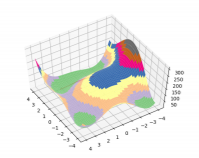
\includegraphics[width=5cm, height=3cm]{./pic/himmelblau.png}
	\caption{himmelblau}
	\end{minipage}
	\begin{minipage}[t]{0.48\textwidth}
	\centering
	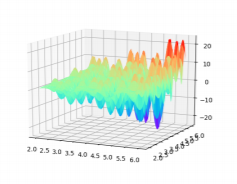
\includegraphics[width=5cm,height=3cm]{./pic/complex_peaks.png}
	\caption{complex peaks}
	\label{complex_peaks}
	\end{minipage}
\end{figure}


关于 himmelblau 函数,容易算出其四个极小值点为 (3,2), (-3.7794,-
3.2832), (3.5845, -1.8481), (-2.8050, 3.1313) 四极值点的中心点几乎是 (0, 0)
点,明显 (0, 0) 点于 (3, 2) 点最近,于是初始化值若为 (0, 0),则优化到的
极值点一般就是 (3, 2)(图例 himmelblau 中红色线条为带动量的 SGD 优化
器优化路线), 但是当你学习率较大,比如 lr=10, 使用 adam,则结果为第二
个极值点,lr=20 时,结果为第三个极值点等。对于 complex\_peaks,观察
其在 $[2, 6] \times [2, 6]$ 区域内的图形,容易看出极值点密集,选取不同初始值并
使用不同的优化器,你会发现很难找到全局的极值点,几乎都停留在初始值
附近的波谷之中。也许神经网络的极值点也大概如此,只是波峰波谷之间的
差距没有 complex\_peaks 函数来得大,但我们仍然要适当跳出局部极值点,
向全局极值点逼近,关于这个问题,我想下一小节的动态调整学习率,会有一
定的帮助 (事实上对鞍点的帮助更大,这点我将利用下一小节的策略,补充
monkey\_saddle 函数的一些实验情况)。

\subsubsection{学习率}
涉及学习率的问题,可以有初始化学习率,学习率的变化策略两点。
对于一个简单的曲面,我们可以根据曲面的一些性质,动态调节学习率,加速收敛,但由于DL高度非凸
且复杂,以及实际应用中的大数据,我们只能在整体上做一些调节,比如熟知的2x step,分步减小,周期性
变化\href{https://arxiv.org/abs/1506.01186}{Cyclical lr},前者假设first step 已经优化到极值点
附近,后者增加了探索性。
最佳初始化学习率,可参考
\label{sub:lr}
\href{https://sgugger.github.io/how-do-you-find-a-good-learning-rate.html}{find start lr}
这里将其改为pytorch1.x版本。
\lstset{style=mystyle}
\begin{lstlisting}[language=Python]

def find_lr(init_value = 1e-8, final_value=10., beta = 0.98):
	num = len(trn_loader)-1
	mult = (final_value / init_value) ** (1/num)
	lr = init_value
	optimizer.param_groups[0]['lr'] = lr
	avg_loss = 0.
	best_loss = 0.
	batch_num = 0
	losses = []
	log_lrs = []
	for data in trn_loader:
		batch_num += 1
		#As before, get the loss for this mini-batch of inputs/outputs
		inputs,labels = data
		inputs, labels = inputs.to(device), labels.to(device)
		optimizer.zero_grad()
		outputs = net(inputs)
		loss = criterion(outputs, labels)
		#Compute the smoothed loss
		avg_loss = beta * avg_loss + (1-beta) *loss.data[0]
		smoothed_loss = avg_loss / (1 - beta**batch_num)
		#Stop if the loss is exploding
		if batch_num > 1 and smoothed_loss > 4 * best_loss:
			return log_lrs, losses
		#Record the best loss
		if smoothed_loss < best_loss or batch_num==1:
			best_loss = smoothed_loss
		#Store the values
		losses.append(smoothed_loss)
		log_lrs.append(math.log10(lr))
		#Do the SGD step
		loss.backward()
		optimizer.step()
		#Update the lr for the next step
		lr *= mult
		optimizer.param_groups[0]['lr'] = lr
	return log_lrs, losses
\end{lstlisting}

这里用 CycleLR,来测试一下上小节给的函数,实验参
数略,实验结果总结起来大致有:针对 complex\_peak 函数,当学习率$ < 1$
时,除 SGD 外各个优化器都很难跳出局部最优;学习率过小且带动量,则
连局部极值点都很难收敛到;学习率大于一定阈值,各优化器均可以跳出
去... ,对于 himmelblau 函数,当其收敛到某一极值点后,各优化器在循环学
习率更新策略下均很难跳出去。以下为梯度更新方向示例图。

\begin{figure}[htbp]
	\centering
	\begin{minipage}[t]{0.48\textwidth}
	\centering
	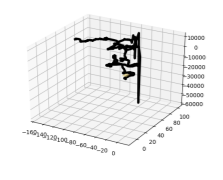
\includegraphics[width=5cm, height=3cm]{./pic/rmsprop_momentum.png}
	\caption{rmsprop momentum}
	\end{minipage}
	\begin{minipage}[t]{0.48\textwidth}
	\centering
	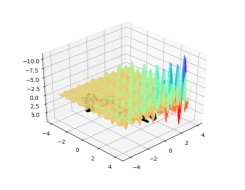
\includegraphics[width=5cm,height=3cm]{./pic/sgd_mometum.png}
	\caption{sgd mometum}
	\label{decent curve}
	\end{minipage}
\end{figure}

想象一下,要想跳出局部极值点,必须增加探索的范围,或者在极值区域附近,疯狂增加学习率,
并记录很多中间结果,然后采用回溯的方式,进行更新。只是这样,代码复杂,速度很慢,而且实际情况是DL
很多极值点的高度都差不多(\ref{all not diff})。


\subsection{post\_processing}
nms包含文字,旋转框,多边形,mask,等,相关描述略,代码可参考本地lib\_functions文件夹。



\section{Detectors}

这节主要分析maskrcnn和reppoints,retinanet三个算法.

\subsubsection{maskrcnn}
\label{maskrcnn}
以配置文件mask\_rcnn\_r50\_fpn\_1x.py为例说说twao\_stage的实现过程.
配合two\_stage的forward\_train()函数和配置文件.

首先backbone为resnet50,(resnet系列结构参见\ref{picresnet}),
其以tuple形式返回4个stage的特征图,片段代码如下:
% \begin{figure}[htbp]
% 	\centering
% 	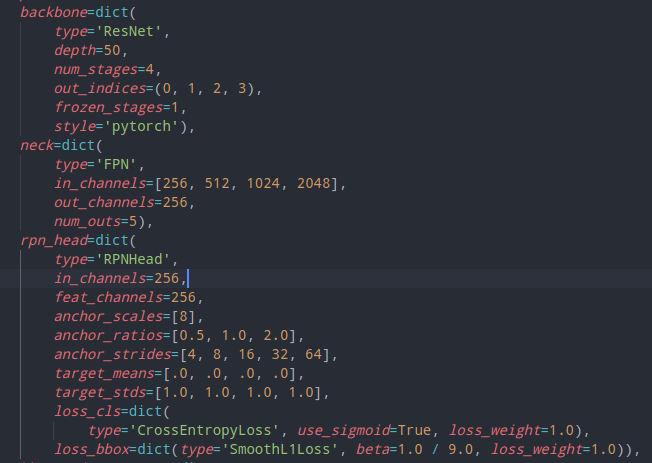
\includegraphics[width=5cm, height=4cm]{./pic/maskrcnn_50.png}
% 	\caption{config maskrcnn}
% \end{figure}
\lstset{style=mystyle}
\begin{lstlisting}[language=Python]

outs = []
for i, layer_name in enumerate(self.res_layers):
	res_layer = getattr(self, layer_name)
	x = res_layer(x)
	if i in self.out_indices:
		outs.append(x)

\end{lstlisting}

然后neck为fpn,结构参见\ref{picfpn},
fpn根据config中的out\_indices取出以resnet50输出的对应stage,分别构造输出channel维度统一的卷积算子,
然后按照\ref{picfpn}所示融合方式进行不同尺度的特征融合,以元组形式输出结果.
在配置信息里有一条num\_outs=5,是为mask-rcnn在最顶层特征增加的最大池化特征输出.以上两块为提取特征,被
extract\_feat整合在一块,

% \lstset{style=mystyle}
% \begin{lstlisting}[language=Python]
% 	for i in range(self.start_level, self.backbone_end_level):
% 		l_conv = ConvModule(
% 			in_channels[i],
% 			out_channels,
% 			1,
% 			conv_cfg=conv_cfg,
% 			norm_cfg=norm_cfg,
% 			activation=self.activation,
% 			inplace=False)
% 		fpn_conv = ConvModule(
% 			out_channels,
% 			out_channels,
% 			3,
% 			padding=1,
% 			conv_cfg=conv_cfg,
% 			norm_cfg=norm_cfg,
% 			activation=self.activation,
% 			inplace=False)

% 		self.lateral_convs.append(l_conv)
% 		self.fpn_convs.append(fpn_conv)

% \end{lstlisting}
紧接着forward\_train中包含了剩下的所有流程.
\begin{equation*}
	\begin{aligned}
		 rpn\_head \rightarrow rpn\_head.loss \rightarrow rpn\_head.get\_bboxes \rightarrow assign \rightarrow sample \\
		\rightarrow bbox\_roi\_extractor \rightarrow  bbox\_head \rightarrow bbox\_head.get\_target. \rightarrow bbox\_h\\
		ead.loss \rightarrow mask\_roi\_extractor \rightarrow mask\_head \rightarrow mask\_head.get\_target
	\end{aligned}
\end{equation*} 

这里梳理一下部分函数.

候选框层RPN,RPNHead继承AnchorHead, 它的几个核心操作都在anchor\_head.py中实现,主要包括get\_anchors, 
anchor\_target见\ref{sub:anchorhead},函数get\_bboxes结合配置参数从rpn前向得到的2分类和位置预测结果中筛选出最终的proposals.

get\_bboxes中先通过self.anchor\_generators[i].grid\_anchors()这个函数取到所有的anchor\_boxs,再
通过self.get\_bboxes\_single()根据rpn前向的结果选出候选框,在self.get\_bboxes\_single()中,先在每个尺度上
取2000(配置)个anchor出来,concat到一起作为该图像的anchor,对这些anchor boxs作nms(thr=0.7)就得到了所需的候选框.
需注意预测的bbox是对数化了的,在做iou计算之前需用delta2bbox()函数进行逆变换.bbox\_head中的bbox2roi类似.

得到的候选框最终由配置中train\_cfg的rcnn.assigner, rcnn.sampler进行标定和筛选,保持正负样本平衡和框的质量,方便优化.

MaxIoUAssigner:
\label{sub:MaxIoUAssigner}
\begin{adjustwidth}{1cm}{0cm}
\begin{itemize}
	\item[1.] 所有候选框置-1
	\item[2.] 将与所有gtbbox的iou小于neg\_iou\_thr置0
	\item[3.] iou大于pos\_iou\_thr的将其匹配
	\item[4.] 为了避免标定框无训练目标,将gtbbox匹配于与它iou最近的bbox(会导致部分正样本的匹配iou值很小).
\end{itemize}
\end{adjustwidth}


\lstset{style=mystyle}
\begin{lstlisting}[language=Python]
	# 交并比矩阵(n,m), gt=n, bboxes=m
	overlaps = bbox_overlaps(gt_bboxes, bboxes)
	# 每个bbox和所有gt的最大交并比,(m,)
	max_overlaps, argmax_overlaps = overlaps.max(dim=0)
	# 每个gt和所有bbox的最大交并比
	gt_max_overlaps, gt_argmax_overlaps = overlaps.max(dim=1)
	# 1将所有bbox赋值为-1,注意new_full操作
	assigned_gt_inds = overlaps.new_full(
			(num_bboxes, ), -1, dtype=torch.long)
	# 2交并比大于0同时小于负阈值的赋值为0
	assigned_gt_inds[(max_overlaps >= 0)
							 & (max_overlaps < self.neg_iou_thr)] = 0
	# 将与gt交并比大于正阈值的赋值为1(可能没有)
	pos_inds = max_overlaps >= self.pos_iou_thr
	assigned_gt_inds[pos_inds] = argmax_overlaps[pos_inds] + 1
	# 保证每个gt至少对应一个bbox
	# 遍历gt,将与gt最近(max(iou))的bbox,将gt的label赋值给此bbox

	for i in range(num_gts):
			if gt_max_overlaps[i] >= self.min_pos_iou:
				# 此判断较迷
				max_iou_inds = overlaps[i, :] == gt_max_overlaps[i]
				assigned_gt_inds[max_iou_inds] = i + 1 
				# 与gt最大iou的bbox 赋值为i+1

\end{lstlisting}

RandomSampler,保持设定的平衡比例,随机采样.

然后通过SingleRoIExtractor(roi\_extractors/single\_level.py)统一RoI
Align四个尺度且大小不同的的proposals,使其大小为7*7(bbox)或14*14
(mask).配置信息rpn\_head中的anchor\_strides为5个尺度,
包含了fpn额外加入的最大池化层,而bbox\_roi\_extractor的featmap\_strides却只包含四个尺度,表明只需对前四层进行align.
最终送入bbox head 和mask head做第二次优化(two stage).

RoIAlign在ops中,经cuda加速,详解略.
其中roi\_extractors中的特征层级映射函数如下:
\lstset{style=mystyle}
\begin{lstlisting}[language=Python]
	def map_roi_levels(self, rois, num_levels):
	"""Map rois to corresponding feature levels by scales.
	 self.finest_scale = 56, 映射到0级的阈值
	$(0, 56, 56*2, 56*4, \infty) \rightarrow (0, 1, 2, 3)$
	bbox2roi变换后的rois

	Returns:
		Tensor: Level index (0-based) of each RoI, shape (k, )
		因不同层级对应不同的ROIAlign
	"""
	scale = torch.sqrt(
		(rois[:, 3] - rois[:, 1] + 1) * (rois[:, 4] - rois[:, 2] + 1))
	target_lvls = torch.floor(torch.log2(scale / self.finest_scale + 1e-6))
	target_lvls = target_lvls.clamp(min=0, max=num_levels - 1).long()
	# 这个变换在原始论文中有.
	return target_lvls
\end{lstlisting}

\subsubsection{RepPoints}

\begin{figure}[htbp]
	\centering
	\begin{minipage}[t]{0.9\textwidth}
	\centering
	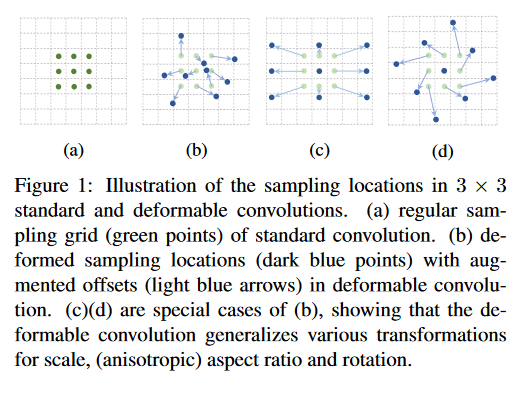
\includegraphics[width=8cm, height=6cm]{./pic/DCN.png}
	\caption{dcn}
	\label{picdcn}
	\end{minipage}
\end{figure}

\begin{figure}[htbp]
	\centering
	\begin{minipage}[t]{0.9\textwidth}
	\centering
	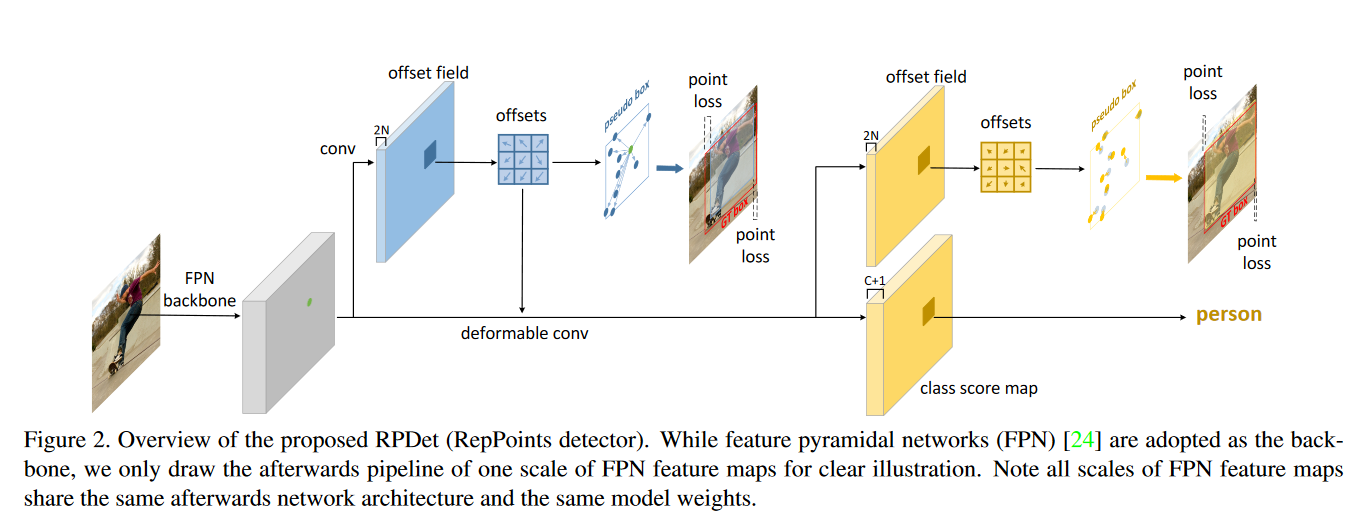
\includegraphics[width=9cm, height=3.2cm]{./pic/RepPoints.png}
	\caption{reppoints}
	\label{picreppoints}
	\end{minipage}
\end{figure}


2019年,Ze Yang等人利用\href{https://arxiv.org/pdf/1811.11168.pdf}{DCNv2}的特性,实现了结构点表示物体的检测算法
\href{https://arxiv.org/pdf/1904.11490.pdf}{RepPoints}。其中DCNv2从DCNv1进化而来,出发点如\ref{picdcn}所示,
改变了卷积的采样点。其卷积数学表达式如下:
$y(p)=\sum_{k=1}^{K} w_{k} \cdot x\left(p+p_{k}+\Delta p_{k}\right) \cdot \Delta m_{k}$
对应的池化层为:$y(k)=\sum_{j=1}^{n_{k}} x\left(p_{k j}+\Delta p_{k}\right) \cdot \Delta m_{k} / n_{k}$
其中$w_k, p, p_k, \Delta p_k, \Delta m_k$分别表示卷积核参数,卷积中心点(图上),当前卷积点,当前点的偏移量,
当前点的权重因子,就这么简单。不规则采样点和图像中物体的不规则形状是吻合的,所以直观上讲,这个卷积是很有意义的。
实验上你可以将以前的conv策略性的替换为dcn,也许会带来性能的提升(ps后续很多新检测算法实验,证明了这一点)。

问题是如何利用DCNv2不规则卷积,来做检测算法呢?

\begin{itemize}
	\item[1.] 通过定位和分类的直接监督来学习可形变卷积的偏移量,使得偏移量具有可解释性(@陀飞轮)。
	\item[2.] 可以通过采样点来直接生成伪框 (pseudo box),不需要另外学习边界框,并且分类和定位是有联系的(@陀飞轮)。
\end{itemize}

从\ref{picreppoints}可以看出,DCN卷积得到$2N$的偏移量,将其限制到标定的bbox,类似于rpn,然后重复DCN得到$2N, C+1$分别作
送入bbox回归和class分类(refine)。也即上面所说的两点。其中的关键点是学习的points,需要限制到标定的bbox中,也即学习的引导。
因为是点表示,所以一个自然的问题是比如人脸检测,那么所得到的点的几何结构是一致的吗?更精细的问题是,可以得到物体的边缘点吗?

这需要对算法更细致的研究了,可以参考一下\href{https://www.zhihu.com/question/322372759/answer/798327725}{官方说明}:

“
这里面“可学习的采样点集合”其实是更本质的概念,这些采样点同时用来提取语义对齐的特征,又用来表示物体的几何形态。
deformable convolution是其中一种基于采样点的特征提取方法,但同时还可以有其它的实现。几何形态监督的方式也可以是更多样的,
除了物体检测中的bounding box标注外,还可以利用更精细的几何标注来进行监督。我们最近有一个工作就提出了不同的特征提取方法,
以及不同的几何监督方式。

通常来说,用anchor去覆盖4d空间是困难的,所以一般需要不同尺度和不同长宽比的多种anchor,而且赋予这个anchor box类别标签也相对麻烦,
需要计算和ground-truth box的IoU。与之对应的,要覆盖2d空间和赋予类别都很容易,典型的2d表示包括center point,corner point等等。

回归vs. 验证是一个很古老的问题,通常来讲求解验证问题比求解回归问题更容易,但是效率更低。在物体检测里面,通常的做法是先做粗验证,
后用回归方法来做精确定位。基于anchor的设计就是典型的验证思路,后续回归只在一个很小的范围内进行。而anchor-free方法更
多依赖回归来求解问题,通常讲更难学习,但是因为有了deep的特征,以及多阶段的定位方法,效果能比肩依赖验证更多的anchor-based
方法,同时框架更简洁。

RepPoints不仅能用来解决物体检测问题,它在表示物体的精细结构上也有很大潜力,例如预测物体的contour(后续会公布)。
”


\subsubsection{Retinanet}
见RetinaHead。


\subsection{Backbone}
\label{backbones}

\begin{figure}[htbp]
	\centering
	\begin{minipage}[t]{0.48\textwidth}
	\centering
	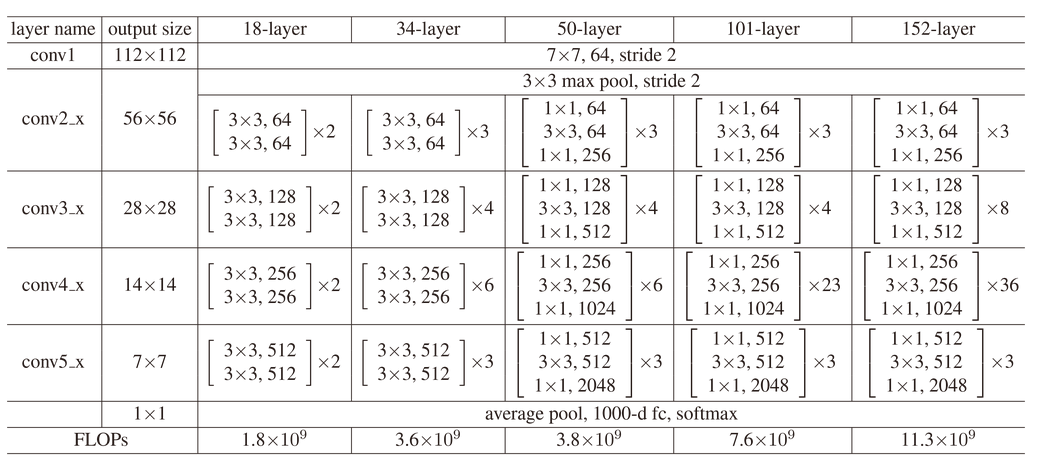
\includegraphics[width=5cm, height=4cm]{./pic/resnet_struct.png}
	\caption{resnet}
	\label{picresnet}
	\end{minipage}
	\begin{minipage}[t]{0.48\textwidth}
		\centering
		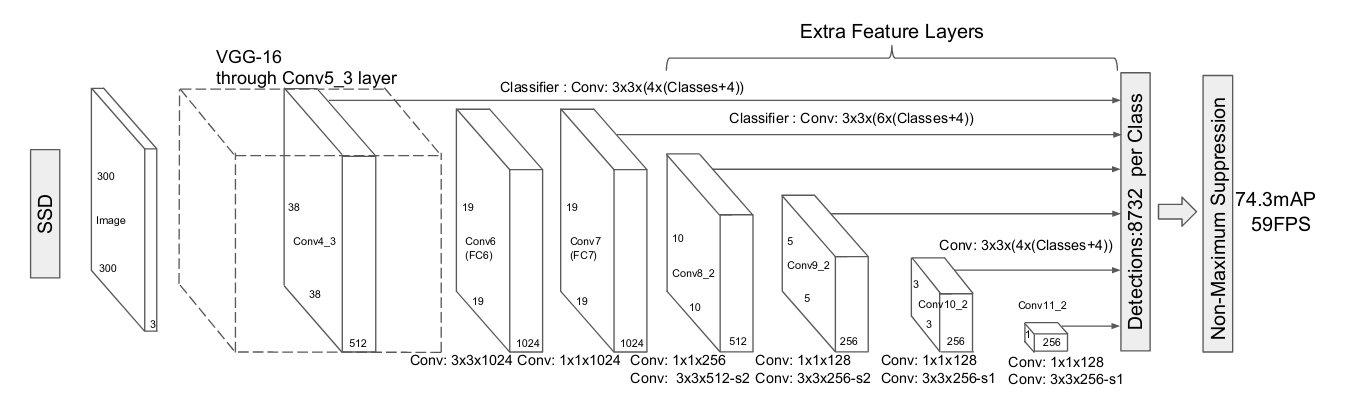
\includegraphics[width=5cm,height=4cm]{./pic/ssd.png}
		\caption{ssd}
		\label{picssd}
	\end{minipage}
\end{figure}

\begin{figure}[htbp]
	\centering
	\begin{minipage}[t]{0.48\textwidth}
	\centering
	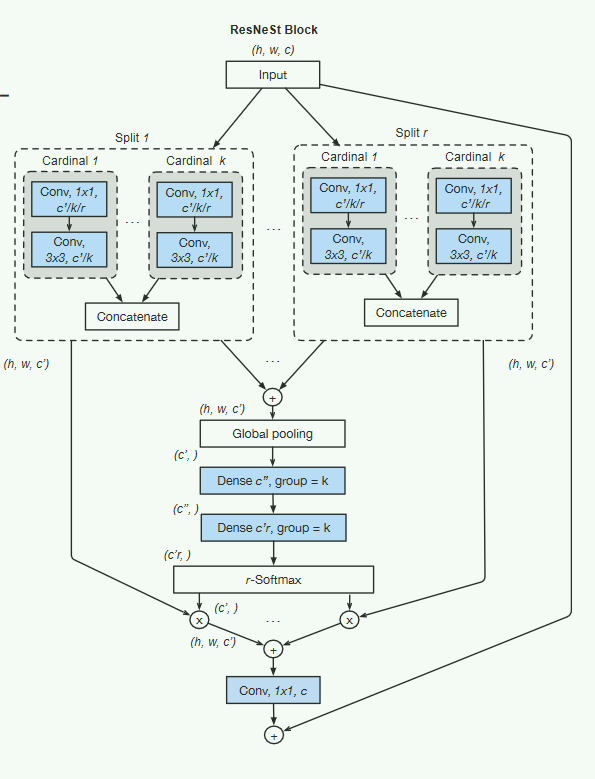
\includegraphics[width=6cm,height=8cm]{./pic/ResNeSt.png}
	\caption{ResNeSt}
	\label{picresnest}
	\end{minipage}
	\begin{minipage}[t]{0.48\textwidth}
		\centering
		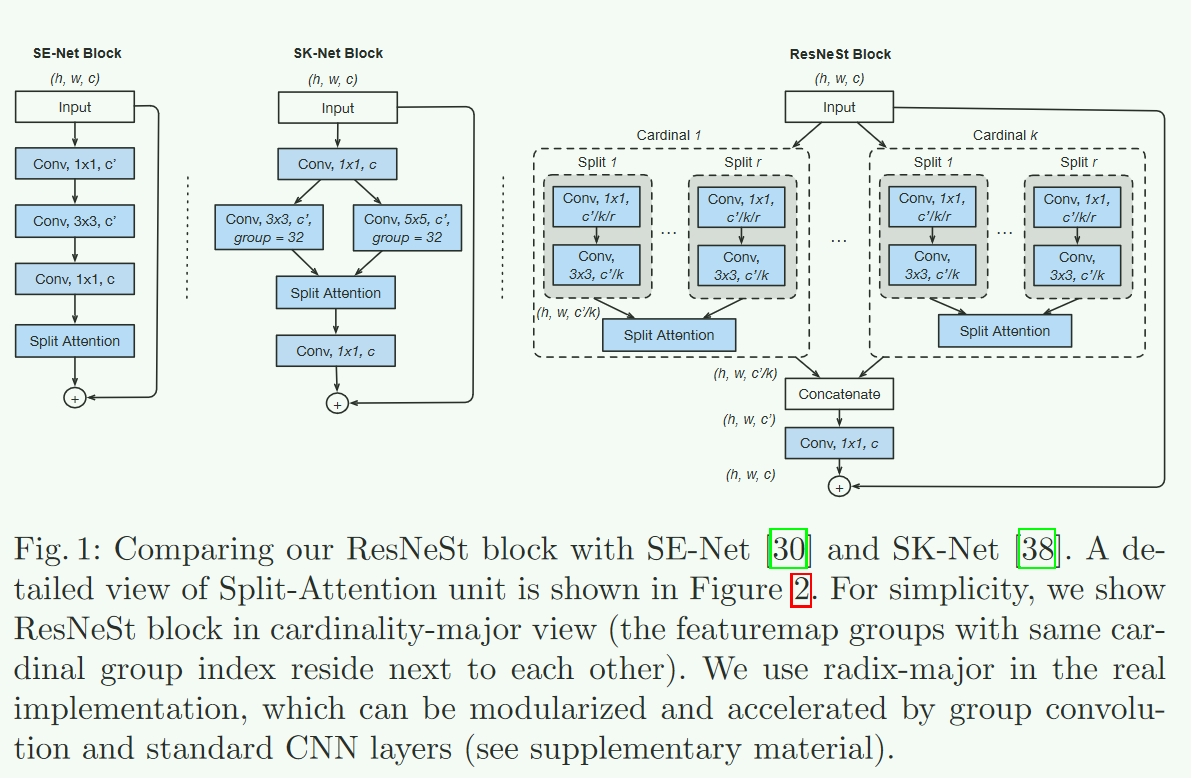
\includegraphics[width=7.5cm,height=5cm]{./pic/ResNeSt_SE_Sk.png}
		\caption{ResNeSt\_SE\_SK}
		\label{picresnest_se_sk}
	\end{minipage}
\end{figure}


\begin{figure}[htbp]
	\centering
	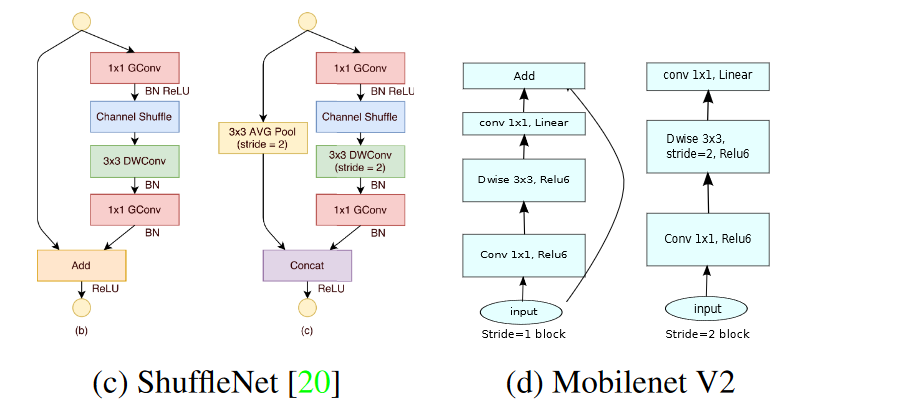
\includegraphics[width=8cm,height=6cm]{./pic/MobileNetV2.png}
	\caption{mobilenetv2}
	\label{picmobilenet}
\end{figure}

\subsubsection{backbone及改进}

出于对\href{https://en.wikipedia.org/wiki/Universal_approximation_theorem}{Universal approximation theorem}的考察,
人们认为加深网络,在复杂问题上会带来更好的效果,但实验情况并非如此,于是
2015年\href{https://arxiv.org/abs/1512.03385}{ResNet}出现,旨在解决模型网络加深带来的性能下降问题(degradation problem)。
其结构参数见\ref{picresnet}。
其中
$
\left[\begin{array}{l}
	3 \times 3,64 \\
	3 \times 3,64
\end{array}\right] 
$
为Basicbolck基础块,
$
\left[\begin{array}{c}
	1 \times 1,64 \\
	3 \times 3,64 \\
	1 \times 1,256
\end{array}\right] 
$
为Bottleneck基础块,后接池化,全连接和
概率softmax映射,Bottleneck计算量为Basicbolck的5.9\%,池化替代全连接,更本质,一来计算量极大减小,二来过滤或者综合
出了更有效的特征。一点需要注意一下,基础块都$\times$了一个数,重复计算可以增加感受野,
同时增加了非线性算算子个数,能提取更抽象的特征,因为上下层尺度只减小了一半,所以stride=2只会在重复块中的某
一个上做操作,这个是可以调节的。

那么ResNet是怎么解决梯度消失问题的呢?由Skip Connection组成的残差块(residual blocks)。

比如将第$l$层到$l+1$层的激活函数改到addition之前(参考\href{https://arxiv.org/abs/1603.05027}{ResNetV2})
的残差模块的表示方式:
$
\mathbf{x}_{l+1}=\mathbf{x}_{l}+\mathcal{F}\left(\mathbf{x}_{l}, \mathcal{W}_{l}\right)
$,
递归形式
$
\mathbf{x}_{L}=\mathbf{x}_{l}+\sum_{i=l}^{L-1} \mathcal{F}\left(\mathbf{x}_{i}, \mathcal{W}_{i}\right)
$,
则其梯度如下:
$$
\frac{\partial loss}{\partial \mathbf{x}_{l}}=\frac{\partial loss}{\partial \mathbf{x}_{L}}
 \frac{\partial \mathbf{x}_{L}}{\partial \mathbf{x}_{l}}=\frac{\partial loss}{\partial 
 \mathbf{x}_{L}}\left(1+\frac{\partial}{\partial \mathbf{x}_{l}} \sum_{i=l}^{L-1} 
 \mathcal{F}\left(\mathbf{x}_{i}, \mathcal{W}_{i}\right)\right)
$$
从BP公式我们知道梯度消失来源于梯度向量叠乘后太小,这里均有+1,极大抑制了梯度消失问题。

ResNet的改进文章有很多,主要可分为模型性能,模型轻量和功能扩展。如上V2,\href{https://arxiv.org/pdf/1812.01187.pdf}{Bag}
包含了性能,轻量上的改进,而\href{https://hangzhang.org/files/resnest.pdf}{resnest}集成了三方面的改进。
resnest结构见\ref{picresnest_se_sk},从结构图基本可以看到该残差模块的含义。现'按图索骥',给出对应的公式(对比论文),
即可完成清晰的理解。

首先对输入特征图按channel分解成$G=KR$部分,其中$K$是cardinal group数,$R$是radix group数,一句话,组中组。
每个原子特征图经过$F_i$映射成$U_i$, $i \in \{1, 2, ..., G\}$。从图中能看到$F_i$为一个$1\times 1, 3 \times 3$卷积组成,
这里好奇为何不是131结构,然后一个$R$小组接一个Split Attention结构,然后$K$个Split Attention 结果concatente在一起和输入图
相加,组成一个残差块。图中有个细节,$c, c'$,这个也是channel降维减小计算量吧(出于这个考虑,也许可以圆一下为何不是131结构)。
$K$个$R$基组经过$F$映射后做求和处理得到$K$基组单位元的表示,$\hat{U}^{k}=\sum_{j=R(k-1)+1}^{R k} U_{j}$,其中
$\hat{U}^{k} \in \mathbb{R}^{H \times W \times C / K}$,每个$K$特征图在channel维度上做一个全局池化得到
该特征图的Global contextual information $s^{k} \in \mathbb{R}^{C / K}$,其中第$c$个channle 
$s_{c}^{k}=\frac{1}{H \times W} \sum_{i=1}^{H} \sum_{j=1}^{W} \hat{U}_{c}^{k}(i, j)$,
这些Global contextual information做一个全连接映射$\mathcal{G}$,得到$K$组中每个$R$组中各特征的channel的重要系数$a_{i}^{k}(c)$,
$$
a_{i}^{k}(c)=\left\{\begin{array}{ll}
	\frac{\exp \left(\mathcal{G}_{i}^{c}\left(s^{k}\right)\right)}{\sum_{j=0}^{R} \exp 
	\left(\mathcal{G}_{j}^{c}\left(s^{k}\right)\right)} & \text { if } R>1 \\
	\frac{1}{1+\exp \left(-\mathcal{G}_{i}^{c}\left(s^{k}\right)\right)} & \text { if } R=1
\end{array}\right.
$$
最后用此系数加权求和$R$组各特征图$U$,其中第$c$ channel为
$V_{c}^{k}=\sum_{i=1}^{R} a_{i}^{k}(c) U_{R(k-1)+i}$,
得到Attention后的$K$组结果,然后concat一下得到映射特征,即$V=\operatorname{Concat}\left\{V^{1}, V^{2}, \ldots V^{K}\right\}$,
最后执行Skip Connection,$Y = V + X$得到残差块的最终输出。$X$上可做操作,可调节。

以上基本囊括了ResNet的改进内容。接着说说mmdet的代码部分。

代码上,Resnet由BasicBlock,Bottleneck,make\_res\_layer构成。其中make\_res\_layer重复构造残差模块。
需要说明的是在resnet.py中引进了dcn,gcb和gen\_attention等功能模块。
从Bottleneck的\_inner\_forward可以看到,gen\_attention\_block加到kerner\_size=1,
kerner\_size=3组(组:卷积,归一化,激活)之后,
kerner\_size=1,planes扩展组之前。
gcb加到planes扩展组之后,然后才是下采样。因dcn是替换卷积算子,其参数和基本卷积相同,因此你可以任意替换conv2d,
只是试验表明,替换此处的kerner\_size=3组效果更好。

代码参数说明,主要和fpn对齐部分,在config中按照如下对齐方式更改即可。
\lstset{style=mystyle}
\begin{lstlisting}[language=Python]

@BACKBONES.register_module
class ResNet(nn.Module):
	arch_settings = {
		18: (BasicBlock, (2, 2, 2, 2)),    # (2, 2, 2, 2)各层残差块的重复数目
		34: (BasicBlock, (3, 4, 6, 3)),
		50: (Bottleneck, (3, 4, 6, 3)),
		101: (Bottleneck, (3, 4, 23, 3)),
		152: (Bottleneck, (3, 8, 36, 3))
	}
	def __init__(self,
					depth,
					in_channels=3,
					num_stages=4,
					strides=(1, 2, 2, 2),
					dilations=(1, 1, 1, 1),
					out_indices=(0, 1, 2, 3),
					style='pytorch',
					frozen_stages=-1,
					conv_cfg=None,
					norm_cfg=dict(type='BN', requires_grad=True),
					norm_eval=True,
					dcn=None,
					stage_with_dcn=(False, False, False, False),
					gcb=None,
					stage_with_gcb=(False, False, False, False),
					gen_attention=None,
					stage_with_gen_attention=((), (), (), ()),
					with_cp=False,
					zero_init_residual=True):
		super(ResNet, self).__init__()
	# num_stages:下采样特征层数目
	# strides:不同残差block的stride数
	# out_indices: 需要的特征层索引,对齐fpn
	# frozen_stages:冻结的残差层
	# stage_with_dcn,stage_with_gcb,stage_with_gen_attention均需要和fpn层对齐

	def forward(self, x):
		# 首先是两个下采样:kernel_size=7和maxpool,此时尺度为原始1/4
		x = self.conv1(x)
		x = self.norm1(x)
		x = self.relu(x)
		x = self.maxpool(x)
		# 然后是几个尺度减半的特征层 make_res_layer,对应fpn层
		outs = []
		for i, layer_name in enumerate(self.res_layers):
			res_layer = getattr(self, layer_name)
			x = res_layer(x)
			if i in self.out_indices:
				# out_indices 选取需要的层对应fpn层(通常index是连续的,除非数据特殊,刚好都只有一大一小物体)
				outs.append(x)
		return tuple(outs)
\end{lstlisting}

说明: resnest被ECCV2020 strong recject了,其中的丰富历史略。

\subsection{Necks}

\begin{figure}[htbp]
	\centering
	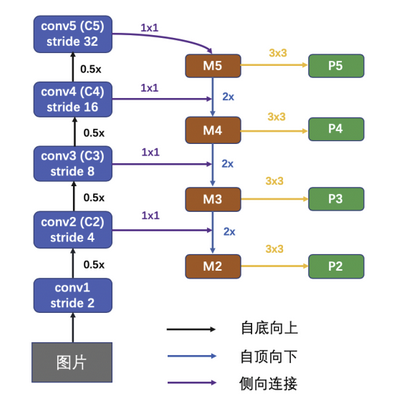
\includegraphics[width=5cm,height=4cm]{./pic/fpn.png}
	\caption{fpn}
	\label{picfpn}
\end{figure}

\begin{figure}[htbp]
	\centering
	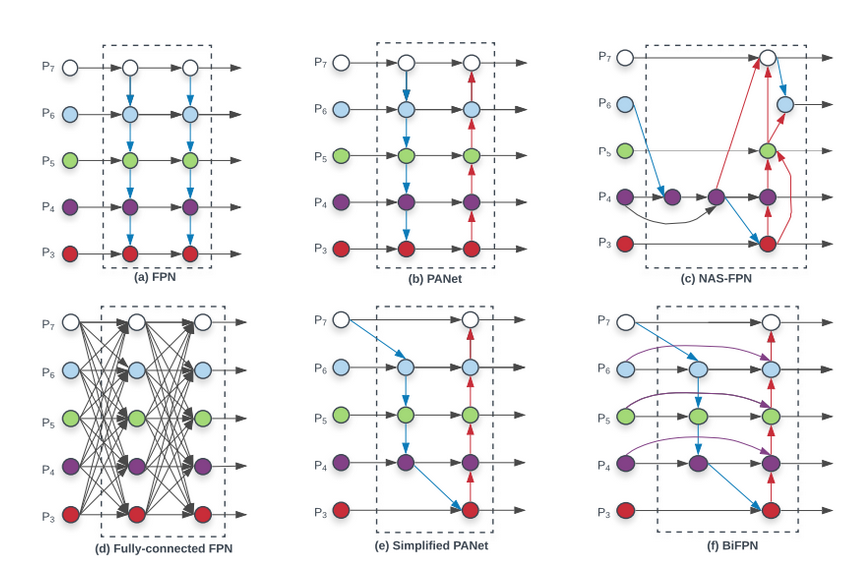
\includegraphics[width=7cm,height=4cm]{./pic/BiFPN.png}
	\caption{bifpn}
	\label{picbifpn}
\end{figure}

\begin{figure}[htbp]
	\centering
	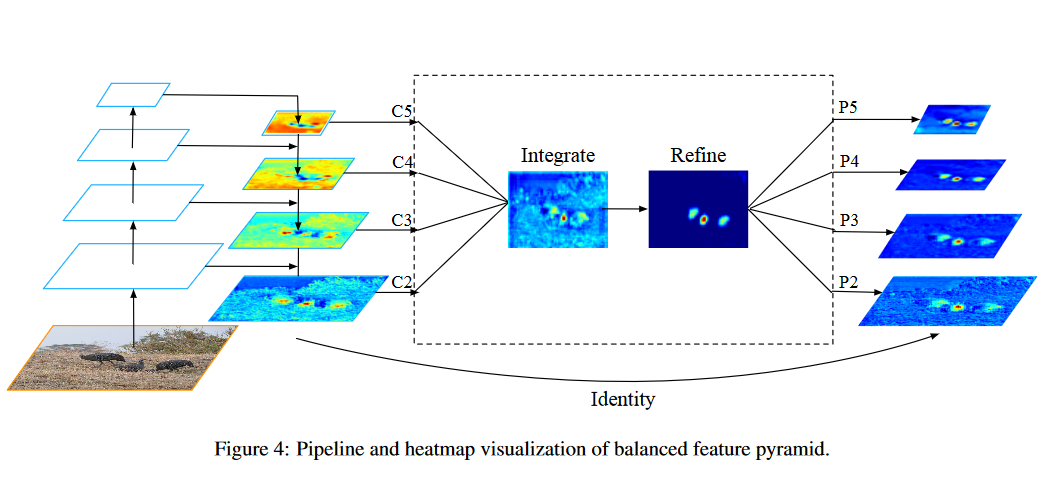
\includegraphics[width=7cm,height=4cm]{./pic/BFPN.png}
	\caption{bfpn}
	\label{picbfpn}
\end{figure}

提到数字图像的多尺度,首先想到的是David Lowe于1999发表的SIFT算法。而DL中的多尺度结构FPN,算了接了SIFT的衣钵。
2017年,Tsung-Yi Lin等人提出\href{https://arxiv.org/abs/1612.03144}{FPN},其摘要中给出解释:
A top-down architecture with lateral connections is developed forbuilding high-level semantic feature maps at all scales。
从中我们看到几个关键词,自顶向下,横向连接,高级语义特征,各种尺度。

想象一下,一张图被1/2下采样了几次,那么同样的物体在不同从尺度上,
表示的信息将至少对半折少(像素信息),那么合并各层信息将有助于有效信息的叠加,抑制某些物体的消失。因此容易看出这几个关键词的一些可变化的地方。
自顶向下,自底向上,连接方式可从全连接开始缩减,获取高级语义特征的方式,不同尺度特征对齐的方式,更多尺度。若采用事后诸葛亮的逻辑,那么后续
确实有一些文章是在围绕这个几个点做改进工作。比如看一眼\ref{picbifpn},不过 \href{https://arxiv.org/abs/1911.09070}{BiFPN}增加了各层的权重因子,
这和后来横飞的Attention是一致的。bifpn的实现参考\href{https://github.com/zylo117/Yet-Another-EfficientDet-Pytorch}{YAEDet.Pytorch},
如果想看更好看的实现,可参考\href{https://github.com/toandaominh1997/EfficientDet.Pytorch/blob/master/models/bifpn.py}{bifpn.pytorch},
实现细节上和论文有出入(YAEDet.Pytorch),所以自行采坑。类似于简化全连接可参考\href{https://arxiv.org/abs/1904.04514}{HRFPN},看图就行,大同小异。
另外mmdet中实现了\href{https://arxiv.org/pdf/1904.02701.pdf}{BFPN},从\ref{picbfpn}可以看到,是对原始fpn后的特征做了一次残差操作。
具体就是特征做了一次合并和解耦(融合,分离),然后和输入特征相加。

fpn的改进远不止以上内容,因为其他很多改进可以合并到\ref{smallobj}小目标改进上,所以这里暂时省去。

最后,FPN的代码相对比较简单,这里选择三点说明。

\lstset{style=mystyle}
\begin{lstlisting}[language=Python]
# 1. 一行代码:
# add extra conv layers (e.g., RetinaNet)
extra_levels = num_outs - self.backbone_end_level + self.start_level

# 参数说明,num_outs:最终fpn输出的尺度个数,backbone_end_level:输入尺度的第几层作为基础fpn输出的最后一层,
# start_level:输入尺度作为基础fpn输出尺度的开始层
# 上面没解释清楚,本来fpn没有额外加层的,你可以理解基础fpn就是原始的fpn,输入多少个层,选一个开始和结束,作为截断就是
#输出结果,现在有了额外层,所以,fpn从基础fpn变为最终fpn。num_outs就是你想输出的最终尺度个数,额外差的尺度特征,从
# 基础fpn被截断的层数(x=backbone_end_level - start_level)末尾开始,往下再下采样y=num_outs-x)即得到最终的fpn特征。

# 2. 一个基础模块: ConvModule,有conv_cfg, norm_cfg,act_cfg三个配置, 作为最小卷积配置单元,注意一下。

# 3. 额外加层:add_extra_convs为False时,Maskrcnn, Fasterrcnn 会在基础fpn上外增加num_outs - used_backbone_levels(x,如上)个max_pool层,
# 为True时,Retina增加额外y层3*3,stride=2的基础ConvModule模块。
\end{lstlisting}

另外经典fpn的自顶向下连接方式从\ref{picfpn}图中容易理解,注意代码中使用的F.interpolate支持3,4,5维的张量。


\subsection{Heads}
head主要处理特征层上的分类和回归任务,它汇集了anchor生成,bbox编码,target设定,以及损失函数的计算。
mmdet v2版本将head分成两部分,one stage的dense\_heads, two stage 的roi\_heads。
因one stage更简单,适用性更好,同时fcos, fovea, reppoints等head需独立实现,所以这里选取
anchor\_head ,retina\_head以做简要说明。

\subsubsection{AnchorHead}
\label{sub:anchorhead}
AnchorHead的基本组成元素在初始化对象时完成,参数信息一目了然。
\lstset{style=mystyle}
\begin{lstlisting}[language=Python]
    @HEADS.register_module()
    class AnchorHead(nn.Module):
        """Anchor-based head (RPN, RetinaNet, SSD, etc.).
        """  
    
        def __init__(self,
                     num_classes,
                     in_channels,
                     feat_channels=256,
                     anchor_generator=dict(
                         type='AnchorGenerator',
                         scales=[8, 16, 32],
                         ratios=[0.5, 1.0, 2.0],
                         strides=[4, 8, 16, 32, 64]),
                     bbox_coder=dict(
                         type='DeltaXYWHBBoxCoder',
                         target_means=(.0, .0, .0, .0),
                         target_stds=(1.0, 1.0, 1.0, 1.0)),
                     reg_decoded_bbox=False,    # 算损失函数时将预测的bbox解码(若True,一般效果不会好吧)
                     background_label=None,
                     loss_cls=dict(
                         type='CrossEntropyLoss',
                         use_sigmoid=True,
                         loss_weight=1.0),
                     loss_bbox=dict(
                         type='SmoothL1Loss', beta=1.0 / 9.0, loss_weight=1.0),
                     train_cfg=None,
                     test_cfg=None):
            super(AnchorHead, self).__init__()

\end{lstlisting}
其中每部分内容已在其他章节说明,在head中,我们只需要关心怎么给anchor打标签,头部网络怎么设计,loss怎么计算,以及如何解析预测结果。
这四部分内容分别见(\_get\_targets\_single, get\_targets),(\_init\_layers), (loss\_single, get\_anchors, loss),
(\_get\_bboxes\_single,get\_bboxes)。其中损失函数见\ref{sec:loss}。

因get\_target, loss 在不同尺度上计算是类似的,于是作者设计了一个公共函数multi\_apply,将同一操作作用于不同尺度上,得到所有
结果。

\lstset{style=mystyle}
\begin{lstlisting}[language=Python]
from functools import partial
from six.moves import map, zip
def multi_apply(func, *args, **kwargs):
    pfunc = partial(func, **kwargs) if kwargs else func
    map_results = map(pfunc, *args)
	return tuple(map(list, zip(*map_results)))
\end{lstlisting}

partial 函数的功能就是:把一个函数的某些参数给固定住,返回一个新的函数(这里就是将**kwargs中的参数固定住).
当函数参数太多,需要固定某些参数时,可以使用 functools.partial 创建一个新的函数
map(function, sequence) ,对 sequence 中的 item 依次执行 function(item),并将结果组成一个 迭代器返回,
最后zip 并行循环.


这里利用\_get\_targets\_single函数来解释multi\_apply函数:

\lstset{style=mystyle}
\begin{lstlisting}[language=Python]
def _get_targets_single(self,
                        flat_anchors,
                        valid_flags,
                        gt_bboxes,
                        gt_bboxes_ignore,
                        gt_labels,
                        img_meta,
                        label_channels=1,
                        unmap_outputs=True):
    """Compute regression and classification targets for anchors in
        a single image.
    """
    # 1. 有效anhcor的index
    inside_flags = anchor_inside_flags(flat_anchors, valid_flags,
                                        img_meta['img_shape'][:2],
                                        self.train_cfg.allowed_border)
    if not inside_flags.any():
        return (None, ) * 6
    # 2. 根据gt和有效anchor采样
    anchors = flat_anchors[inside_flags, :]
    # assign 见core章节
    assign_result = self.assigner.assign(
        anchors, gt_bboxes, gt_bboxes_ignore,
        None if self.sampling else gt_labels)
    sampling_result = self.sampler.sample(assign_result, anchors,
                                            gt_bboxes)
    
    # 3. 构造损失函数计算变量                                        
    num_valid_anchors = anchors.shape[0]
    bbox_targets = torch.zeros_like(anchors)
    bbox_weights = torch.zeros_like(anchors)
    labels = anchors.new_full((num_valid_anchors, ),
                                self.background_label,
                                dtype=torch.long)
    # 3.1 label_weights: 记录张量上需要被计算的点,细节见损失函数章节
    label_weights = anchors.new_zeros(num_valid_anchors, dtype=torch.float)
    # 3.2 对采样后的anchor做一些编码
    pos_inds = sampling_result.pos_inds
    neg_inds = sampling_result.neg_inds
    if len(pos_inds) > 0:
        if not self.reg_decoded_bbox:
            pos_bbox_targets = self.bbox_coder.encode(
                sampling_result.pos_bboxes, sampling_result.pos_gt_bboxes)
        else:
            pos_bbox_targets = sampling_result.pos_gt_bboxes
        bbox_targets[pos_inds, :] = pos_bbox_targets
        bbox_weights[pos_inds, :] = 1.0
        ...

    # 4. 将anchor unmap 回原图
    ...

    return (labels, label_weights, bbox_targets, bbox_weights, pos_inds,
            neg_inds)
            
# 在 get_targets中
# 调用\_get\_targets\_single函数之前
num_imgs = len(img_metas)
assert len(anchor_list) == len(valid_flag_list) == num\_imgs
# anchor number of multi levels
# 选出第一张图的各个特征层的anchor数量,比如上面给的p2即为160*160*6,一格点对应的anhor shape为(6,4)
# 因为有多层,比如p2,p3,则[(160*160*4,4), (80*80*6,4)]
# 为images_to_levels函数,切片用:将所有以图片为第一维度的结果,转换成以特征图尺度个数为第一维度的结果(算loss)
num_level_anchors = [anchors.size(0) for anchors in anchor_list[0]]
# concat all level anchors and flags to a single tensor
#在调用multi\_apply之前需要将anchor\_list的不同层级的anchor cat在一起,最终变为list[Tensor]结构.
#最外层为图像个数.这样就能利用multi\_apply中的map在每张图上做做同样的操作了.
#将所有图的anchor合在一起
for i in range(num_imgs):
	assert len(anchor_list[i]) == len(valid_flag_list[i])
	anchor_list[i] = torch.cat(anchor_list[i])
	valid_flag_list[i] = torch.cat(valid_flag_list[i])
    # valid_flag_list结合meta信息,进一步筛选无效anhor(其实筛掉的很少)

# 然后调用_get_targets_single
result = multi_apply(
        self._get_targets_single,,
        concat_anchor_list,
        concat_valid_flag_list,
        gt_bboxes_list,
        gt_bboxes_ignore_list,
        gt_labels_list,
        img_metas,
        label_channels=label_channels,
        unmap_outputs=unmap_outputs)

(all_labels, all_label_weights, all_bbox_targets, all_bbox_weights,
pos_inds_list, neg_inds_list) = results[:6]

# 最后调用images_to_levels 将 target 按level排序(不同尺度的target会记录相应的anchor个数,作为level分界线)
\end{lstlisting}

此时multi\_apply的*args参数:
\begin{itemize}
    \item concat\_anchor\_list:get\_anchor而得,是一个list[list[Ten
    sors]]结构,最外层是图片个数,再内一层是尺度个数,里面的Tensors的shape是[H*W*K, 4],
    其中H和W代表对应尺度特征图的高和宽.
	\item img\_metas有五个字段:ori/img/pad\_shape, scale\_factor, flip
	
\end{itemize}

\lstset{style=mystyle}
\begin{lstlisting}[language=Python]
@force_fp32(apply_to=('cls_scores', 'bbox_preds'))
def loss(self,
            cls_scores,
            bbox_preds,
            gt_bboxes,
            gt_labels,
            img_metas,
            gt_bboxes_ignore=None):
    featmap_sizes = [featmap.size()[-2:] for featmap in cls_scores]
    assert len(featmap_sizes) == self.anchor_generator.num_levels

    device = cls_scores[0].device
    # 1.生成anchor
    anchor_list, valid_flag_list = self.get_anchors(
        featmap_sizes, img_metas, device=device)
    label_channels = self.cls_out_channels if self.use_sigmoid_cls else 1
    # 2. 标定anchor
    cls_reg_targets = self.get_targets(
        anchor_list,
        valid_flag_list,
        gt_bboxes,
        img_metas,
        gt_bboxes_ignore_list=gt_bboxes_ignore,
        gt_labels_list=gt_labels,
        label_channels=label_channels)
    if cls_reg_targets is None:
        return None
    (labels_list, label_weights_list, bbox_targets_list, bbox_weights_list,
        num_total_pos, num_total_neg) = cls_reg_targets
    num_total_samples = (
        num_total_pos + num_total_neg if self.sampling else num_total_pos)

    # anchor number of multi levels
    num_level_anchors = [anchors.size(0) for anchors in anchor_list[0]]
    # concat all level anchors and flags to a single tensor
    concat_anchor_list = []
    for i in range(len(anchor_list)):
        concat_anchor_list.append(torch.cat(anchor_list[i]))
    all_anchor_list = images_to_levels(concat_anchor_list,
                                        num_level_anchors)

    losses_cls, losses_bbox = multi_apply(
        self.loss_single,
        cls_scores,   # init_layers 网络头部预测, 调用forward_single
        bbox_preds,  # init_layers 网络头部预测
        all_anchor_list,
        labels_list,
        label_weights_list,
        bbox_targets_list,
        bbox_weights_list,
        num_total_samples=num_total_samples)
    return dict(loss_cls=losses_cls, loss_bbox=losses_bbox)


\end{lstlisting}


\subsubsection{SSDHead}
ssd结构的检测网络,目前已有ssd300,ssd512,结构细节参考\ref{picssd}. 从配置文件中可有看到,它没有neck,
因层级结构在backbone实现.

ssdhead继承自anchorhead,主要功能为处理多层级特征上的anchor构造和target标定与筛选,
基本的feauturemap上的acnhor生成由mmdet.core.
anchor中的AnchorGenerator完成,优化目标anchor由anhor\_target完成.
ssdhead中forward前向返回各层级对应的类别分数和坐标信息,loss函数则得到对应的损失函数,以字典的形式返回,最终求导时,汇总成一个值,同时也能计算各个部分损失函数的均值,方差,方便优化,debug.

此处的难点在于anchor的设定和target的标定,筛选.现就anchor这一块细说如下:

anchor基本介绍: anchor设计和caffe ssd anchor设计一致, 假设min\_size为$a$, max\_size为$b$, 则先生成ratio为1, 宽度和高度为$(a, a), (\sqrt{ab}$, 
$\sqrt{ab})$的两个anchor, ratio为$2, 1/2, 3, 1/3$则分别生成宽度和高度为$(a*\sqrt{ratio}, a/\sqrt{ratio})$的anchor, mmdetection中必须设定每一层的min\_size, max\_size, 因此ratios为$[2]$则对应4个anchor, ratios为$[2,3]$则对应6个anchor.

在init()函数中,先生成min\_size, max\_size, 注意它这里是必须要指定max\_size(和caffe SSD不同,无法生成奇数个anchor), 确保len(min\_size)=
len(max\_size), 调用AnchorGenerator()类生成了base\_anchors, 数量是6或者10,使用indices操作从6个anchor里选择$(0, 3, 1, 2)$或者从10个anchor里选择$(0, 5, 1, 2, 3, 4) $$\rightarrow$ 最终生成4个或者6个anchor.于在多个feature map上生成anchor,因此使用了一个for循环操作, 将anchor\_generator放入到anchor\_generatos[]中.


AnchorGenerator类, init()函数需要如下参数:

\begin{itemize}
	\item base\_size: 即设置的min\_size
	\item scales: 是$(1, \sqrt{max\_size / min\_size})$, 用来生成ratio为1的两个anchor
	\item ratios: 是$(1, 2, 1/2)$或者$(1, 2, 1/2, 3, 1/3)$
	\item ctr: ctr由stride生成, 是anchor的中心坐标, $(\frac{stride - 1}{2}, \frac{stride - 1}{2} ) $在gen\_base\_anchor()函数里, 使用上面的参数来计算base\_anchor, 计算流程如下:
	\begin{itemize}
		\item 根据ratios来计算h\_ratios和w\_ratios, 即上面所述的$(1 / \sqrt{ratios}$, $\sqrt{ratios}) $.
		\item 根据scales来计算base\_size, 一共有2个分别是$$(min\_size, \sqrt{min\_size * max\_size}) = min\_size * scales$$
		\item 计算anchors的宽度和高度, 只以宽度举例: $w = base\_size * w\_ratios$, 以ratios是$(1, 2, 1/2)$举例, base\_size shape为$(2, 1)$, w\_ratios shape为$(1, 3)$, 
		计算出的w是$(2, 3) $一共生成了6个anchor, 如果ratios是$(1, 2, 1/2, 3, 1/3)$, 则生成10个anchor (此处anchor数量和标准ssd anchor数量不一致 $\rightarrow$
		 再筛选(即ssd\_head.py中使用indices操作进行筛选))
	\end{itemize}
	
\end{itemize}

说明: 此为1.x版本。

\subsubsection{RetinaHead}
RetinaHead继承AnchorHead,只需要实现\_init\_layers和forward\_single即可,这点retina\_head一看即明。
需要额外注意一点的是,retina在fpn后增加了几层ConvModule。

\subsubsection{FCOSHead}
\label{sub:FCOSHead}
fcoshead并非继承anchorhead,代码得从0解析,故略。

这里补一点fcos的论文简略解读(每个算法细节都很多,具体实践也会有大量的额外trick,并非一点文字可以说明,具体坑还得自愿踩)。

物体检测的算法基本可以用以下这段话来描述:

在某一度量(..)下,找出与人为标定的物体的框的集合,利用这个集合按不同策略生成更有效的正负样本,完成物体的位置预测.

以IOU为度量的模型有Faster R-CNN, SSD 和 YOLOv2, v3等.
它从标定框与虚拟框的偏移集中学习物体的标定框与虚拟框的映射关系,以此来完成物体定位.这里的隐含点为映射变量为物体的表示向量,
这是根据类别标签优化而得. FCOS可以称为以center-ness为度量的检测模型.它将标定框内的聚中心的所有点作为物体的有效表示点,
学习其与标定框的中心偏移量,完成物体的检测.

因为两者度量方式不同,导致后续操作差别比较大,iou度量的
anchor-based模型,需要给每个位置点设计不同形状的anchor作为候选框,然后在所有尺度上进行筛选(或不同尺度分别筛选),
这个过程较为细致,且超参数较多,对不同任务较为敏感.后者anchor-free则省去了anhor构造的过程,可以直接在选出的点上做位置偏移预测,比较简单.


\begin{figure}[htbp]
	\centering
	\begin{minipage}[t]{0.9\textwidth}
	\centering
	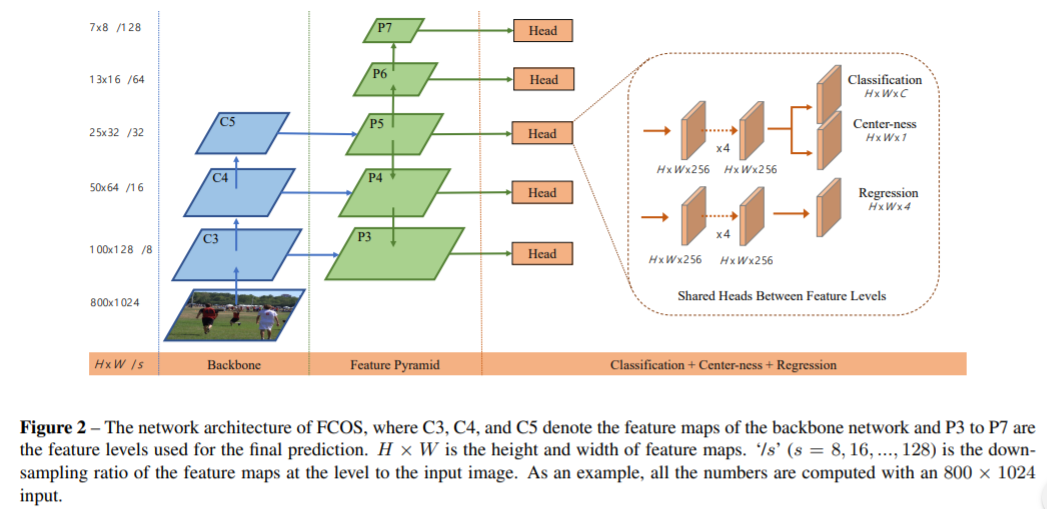
\includegraphics[width=5cm, height=4cm]{./pic/fcos_struct.png}
	\caption{fcos}
	\label{picfcos}
	\end{minipage}
\end{figure}

从以上结构图能清晰的看到FCOS算法的的三大模块.它的核心点在Classification + Center-ness + Regression.
(代码以maskrcnn-benchmark为基础,核心在rpn/fcos的三个文件中(后续).)

这里有几点需要说明:
\begin{itemize}
    \item 限制不同特征层的预测框范围
    $\left\{P_{3}, P_{4}, P_{5}, P_{6}, P_{7}\right\}$对应范围
    区间$0,64,$ $128,256,512 \text { and } \infty$.
    
    \item $P_i, \text{层的位置回归做如下动态调整}\exp \left(s_{i} x\right)$以适应不同特征层回归不同范围.
    
    \item 位置预测的是中心点距离物体左上下右的距离,且位置回归函数是UnitBox中的IOU loss.
    
    \item IOU loss:
    $
	\begin{array}{l}{\square \text { Ground that } \tilde{x}=\left(\tilde{x}_{t}, x_{b}, \tilde{x}_{l},
		\tilde{x}_{r}\right)} \\ {\square \text { predictors } \quad x=\left(x_{t}, x_{b}, x_{l}, x_{r}\right)} \\
		{\ell_{2} \text { loss }=\|\square-\square\|_{2}^{2}} \\ 
	{\text { IoU loss }=-\ln \frac{\text {Intersection}(\square, \square)}{\text {Union}(\square, \square)}}
	\end{array}$
    
    \item $\text { centerness }^{*}=\sqrt{\frac{\min \left(l^{*}, r^{*}\right)}{\max \left(l^{*}, r^{*}\right)} \times \frac{\min \left(t^{*}, b^{*}\right)}{\max \left(t^{*}, b^{*}\right)}}$ 以此来筛选更有代表的物体表示点.
    
    \item 在多个box内的点,选择box 面积最小的那个作为其label box.
    
\end{itemize}

最终损失函数为:
$$
\begin{aligned} L\left(\left\{\boldsymbol{p}_{x, y}\right\},
\left\{\boldsymbol{t}_{x, y}\right\}\right) &=\frac{1}{N_{\mathrm{pos}}} 
\sum_{\boldsymbol{x}, y} L_{\mathrm{cls}}\left(\boldsymbol{p}_{x, y}, c_{x, y}^{*}\right) 
\\ &+\frac{\lambda}{N_{\mathrm{pos}}} \sum_{x, y} \mathbb{I}_{\left\{c_{x, y}^{*}>0\right\}} 
L_{\mathrm{reg}}\left(\boldsymbol{t}_{x, y}, \boldsymbol{t}_{x, y}^{*}\right)
 \end{aligned}
$$

\subsection{Losses}
\label{sec:loss}
\subsubsection{基本认识}

\href{https://arxiv.org/abs/1708.02002}{Fcoalloss}.
想像一下特征层上的锚框,远离gt的必然占绝大多数,围绕在gt周围的bbox有模棱两可的(正负),故有正负难易之分.
FcoalLoss 是为解决难易样本的不平衡问题.公式如下:
\begin{equation}
	FL(p_t) = -\alpha_{t}(1-p_t)^{\gamma}log(p_t),\text{其中}
	p_t=\left\{
	\begin{aligned}
	&p & if y =1\\
	&1-p & else.
	\end{aligned}
	\right.
\end{equation}

$\alpha_t$缓解样本不平衡现象,$(1-p_t)^{\gamma}$为降低易分样本的损失值(考虑到易分样本比例高).
公式可以这样理解:对于正样本分对了,则$p_t->1$,$(1-p_t)^{\gamma}$有减缓效果,当分错了,即
$p_t << 0.5$,则$1-p_t >>0.5$,效果和CrossEntropy没差,对于负样本也是如此.因此起到压缩
图6中的左图右端,右图左端的效果.

\begin{figure}[htbp]
	\centering
	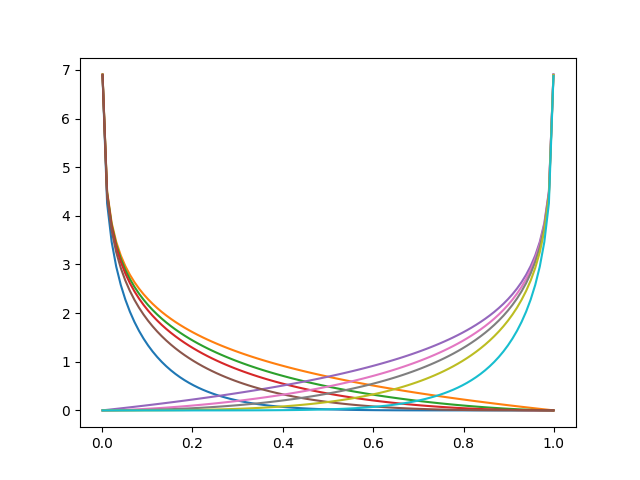
\includegraphics[width=5cm,height=3cm]{./pic/Focal_01.png}
	\caption{FcoalLoss}
\end{figure}

\href{https://arxiv.org/abs/1811.05181}{GHM}.
GHM算是对Fcoal改进,作者统计了样本的梯度信息,提出梯度均衡机制,让各种难度类型的样本有均衡的累计贡献.具体细节看论文即可.

\href{https://arxiv.org/abs/1908.03851}{IoULoss}.
\href{https://arxiv.org/abs/1711.00164}{BoundedIoULoss}.

\subsubsection{实现解析}
mmdet.models.losses里面实现了所有损失函数。

losses.utils有两个基本函数,weight\_reduce\_loss和weighted\_loss,前者将返回的损失向量点乘一权重向量,再分别求和或者算平均值。后者为一
装饰器,装饰你自己定义的损失函数,实现带权重效果。具体为先算自定义loss\_func,然后再weight\_reduce\_loss一下。其中weighted\_loss中
的@functools.wraps装饰的好处是返回的函数保持被装饰函数名字。接下来逐一说明各个损失函数。

CrossEntropyLoss,其理论来源有两点,信息论或极大似然估计,可参考花书。
pytorch官方文档给的公式,明显看出是极大似然的写法。注意实际运算是张(向)量的形式。
$\operatorname{loss}(x, \text { class })=-\log \left(\frac{\exp (x[\text { class }])}{\sum_{j} \exp (x[j])}\right)=
-x[\text { class }]+\log \left(\sum_{j} \exp (x[j])\right)$,增加权重因子为
$$\operatorname{loss}(x, \text { class })=
w e i g h t[\text { class }]
\left(-x[\text { class }]+\log \left(\sum_{j} \exp (x[j])\right)\right).$$
在cross\_entropy\_loss.py中实现了三种交叉熵损失函数,binary\_cross\_ent
ropy, mask\_cross\_entrop以及cross\_entropy,前两者相同点在于将标签扩展成one hot形式
然后调用F.binary\_cross\_entropy\_with\_logits函数,不同点为mask没有乘权重向量,cross\_entropy调用
F.cross\_entropy,并被weight\_reduce\_loss了。
需要注意的点是,最终的CrossEntropyLoss中的loss\_weight参数是多任务中此Loss的权重。而weight\_reduce\_loss
中的weight是各类别的权重。可以说前者和样本平衡有关,后者和任务平衡有关。

SmoothL1Loss来源于FastRCNN,用于解决方框回归的不稳定问题(也许是优化速度),由L2,L1演变而来。
$$L_{1}=\begin{array}{l}
	0.5 x^{2}, \quad|x|<1 \\
	|x|-0.5, \quad x<-1 \text { or } x>1
	\end{array}$$
三者的关系,画个图其意自明:L2两边变化太快,对不好优化的anchor不友好(离群点),L1 0点不可导,Smooth两边较为平缓。
在smooth\_l1\_loss.py中,smooth\_l1\_loss被上述weighted\_loss装饰,
实现代码比较简单:
\lstset{style=mystyle}
\begin{lstlisting}[language=Python]
diff = torch.abs(pred - target)
loss = torch.where(diff < beta, 0.5 * diff * diff / beta,
				   diff - 0.5 * beta)
\end{lstlisting}
注意这里的where实现了分段函数,所以其含义自明。

BalancedL1Loss来自Libra R-CNN,为SmoothL1的改进。
改进函数为
$$
L_{b}(x)=\left\{\begin{array}{ll}
	\frac{\alpha}{b}(b|x|+1) \ln (b|x|+1)-\alpha|x| & \text { if }|x|<1 \\
	\gamma|x|+C & \text { otherwise }
	\end{array}\right.
$$
其梯度为:
$$
\frac{\partial L_{b}}{\partial x}=\left\{\begin{array}{ll}
	\alpha \ln (b|x|+1) & \text { if }|x|<1 \\
	\gamma & \text { otherwise }
	\end{array}\right.
$$
其中$b=e^{\frac{\gamma}{\alpha}}$,使得函数连续。容易得到在 $|x|<1$ 附近的梯度比SmoothL1要大。
具体分析可参考\href{https://zhuanlan.zhihu.com/p/64541760}{BalancedL1Loss},代码和SmoothL1一致,故析略。

Fcoalloss原理见上节,其扩展有\href{https://arxiv.org/pdf/1904.07850.pdf}{CenterNet},GHM系列。
因\_sigmoid\_focal\_loss由cpp,cu实现,故略(可看看debug版本)。 

GHMLoss有GHMC, GHMR,分别作用于分类,回归。原理查看论文或者参考\href{https://zhuanlan.zhihu.com/p/80594704}{GHM},
其主要思想是简单和特难的样本均进行抑制,也算是FocalLoss的改进,析码略。

剩下的IoULoss,BoundedIoULoss,GIoULoss等以iou的方式进行Box回归,含义自现。
三者的细致分析(各自优缺点及关系)看原始论文。代码上根据如下公式,即可容易写出。
Giou:
\begin{equation*}
\begin{array}{l}
	I o U=\frac{|A \cap B|}{|A \cup B|} \\
	G I o U=I o U-\frac{|C \backslash(A \cup B)|}{|C|}
	\end{array}
\end{equation*}其中$C$为$A, B$的闭包。
在iou\_loss.py中,最终的iou\_loss为$-log(ious)$, giou\_loss为$1-gious$
, boundedloss和SmoothL1Loss差不多,只是此时被求的变量$(dx,dy,dw,dh)$的编码方式变了。
具体关系如下:

论文中的分段函数为Huber loss
$
L_{\tau}(z)=\left\{\begin{array}{cc}
	\frac{1}{2} z^{2} & |z|<\tau \\
	\tau|z|-\frac{1}{2} \tau^{2} & \text { otherwise }
	\end{array}\right.
$
和SmoothL1类似,但代码用的是带了一个$\beta$因子的SmoothL1。

分量损失为
$
\text { cost }_{\mathrm{i}}=
2 L_{1}\left(1-\mathrm{I} \mathrm{o} \mathrm{U}_{\mathrm{B}}\left(i, b_{t}\right)\right)
, i \in \{x, y, w, h\}.$
原始的$L1$(见FasterRCNN)定义为
$$
\begin{aligned}
	&\operatorname{cost}_{x}=L_{1}\left(\frac{\Delta x}{w_{s}}\right)\\
	&\operatorname{cost}_{\mathrm{w}}=L_{1}\left(\ln \left(\frac{w}{w_{t}}\right)\right)
	\end{aligned}
$$
这里使用的
$\mathrm{IoU}_{\mathrm{B}}$定义为:
$$
\begin{array}{l}
	\operatorname{IoU}_{\mathrm{B}}\left(x, b_{t}\right)=\max \left(0, \frac{w_{t}-2|\Delta x|}{w_{t}+2|\Delta x|}\right) \\
	\operatorname{IoU}_{\mathrm{B}}\left(w, b_{t}\right)=\min \left(\frac{w}{w_{t}}, \frac{w_{t}}{w}\right)
	\end{array}.
$$
最终分别算出$x,y,w,h$的各自$IoU_B$"损失",作为最终损失的分量,带入SmoothL1分段函数中即可。


以上的代码中出现了new\_full,nonzero,numel,expand,where等常用函数。


\section{简单实践}
\subsection{更改模型}
\subsubsection{增加模块}
本身就包含了很多更改配置文件。
\subsubsection{模型瘦身}
已有模型参数思路:各自参数往小的方向改,比如结构的重复次数,channel的数目,或者采用更多的$1*1$替换$3*3$,甚至可使用$m*n $联合
$n*m$替换$m*m$卷积等。检测模型基本组件(mmdet中的理解)替换:backbone更改为熟知的轻量backbone,比如mobilev2。自行设计思路:这
就考虑任务特性,自身对模型的认识水平和经验问题了,后面补充一个样例,作为参考。


\subsection{抽离模型}
\subsubsection{retinanet\_resnet18}
只需要将需要的部分代码抽离出来,作为单独的inference模型,可参考本地代码retinanet\_resnet18。

\subsection{新增模型}
\subsubsection{centernet}
\label{sub:centernet}
先看原始论文Objects as Points以及官方代码。
然后mmsdet/centernet/core 下的gaussian\_radius函数的解读可参考
\href{https://zhuanlan.zhihu.com/p/96856635}{centernet heatmap解读},
对推广的FocalLoss的更细致的分析可参考
\href{https://zhuanlan.zhihu.com/p/66048276}{centernet解读},
想做一些其他任务尝试的可参考
\href{https://zhuanlan.zhihu.com/p/76378871}{centernet 一些尝试}。

\subsubsection{代码说明}
这里只是将mmdet的注册方式和配置文件类拿来用了一下,
从原始代码\href{https://github.com/xingyizhou/CenterNet}{centernet office code}
将需要的部分抽离出来,将pose模型改成了backbone+heathead结合成HeatMap的形式,其他文件做了和自己对mmdet的理解保持一致方面的些调整。
很多部分没有按照mmdet的方式去改写,想了下改动有点大,数据,pipeline,训练方式等,就算了。

datasets将原始的数据类\_\_getitem\_\_分开实现的方式合并了,原始这样实现主要是不同的方向不同的getitem所致吧。ops里的dcn等就没有加进来了。
这个有参考抽离模型一节。

一些说明点:
\begin{itemize}
	\item[0] 没有fpn, resnet的stem\_layer出来后,做了三次下采样,然后又三次转置卷积回去了,也就是得到了heatmap特征图。
	\item[1] dcn替换在转置卷积部分
	\item[2] detector中的base\_detector, cdetdector只是用来测试的
	\item[3] loss 的实现上,张量的选取 tensor[index] 没有tensor * mask速度快
	\item[4] 核心地方在core中,这和mmdet中anchor相关的意思一致,core/imgage.py中的射影点是原始图scale后的中心点,中心点关于scale/2左移,
	以及这两点关于图像原点组成的一个三角形(见get\_3rd\_point)。
	\item[5] \_\_getitem\_\_中将输入图像射影到(512, 512)大小(2**n),然后在构造的512/4=128大小的heatmap mask上赋值对应的hm,wh,reg,
	其中hm是将原始框射影到128大小的heatmap mask上,根据对应的框中心,进行赋值;wh就是射影后的w,h值,reg为中心向上取整后的误差,也即中心偏移量。
\end{itemize}

整体上centernet的思想是非常简洁的,效果也很好,以及后续的centertrack的end2end式追踪方案,不过后者的前后帧处理方式优化点似乎较多。
\subsection{numpy,torch某些基础函数}
\label{sec:basefunc}

\begin{itemize}
    \item 损失函数部分 \begin{itemize}
        \item torch相关:new\_full,nonzero,numel,expand,where:分段函数。
    \end{itemize}
    \item 模型评估部分 \begin{itemize}
        \item numpy相关:cumsum,finfo,vstack,hstack,concatenate,argmax,
        \item argsort,zeros\_like,newaxis
        \item torch相关:type\_as,stack,x[:,None]*y[None,:],contiguous,view,
        \item max(和numpy的区别)
    \end{itemize}
    \item 其他
    \begin{itemize}
        \item permute, transpose
    \end{itemize}
\end{itemize}


\section{检测模型的简略综述}
检测算法是由一些基本的组件组合而成.这也是mmdection出现的原因.这章节会在不同算法系列中总结一些基础组件,最后再做个提取.
\subsection{通用物体检测}
按照物体编码方式可分为三类.矩形编码(anchor机制),结构点编码(RepPoints)和所有点编码(mask).
\subsubsection{Yolo系列}
yolo相对孤立,v1就不说了,v2,v3基本思想还是来源于resnet,fpn,ssd等.
代码可参考 \href{https://github.com/ultralytics/yolov3}{yolov3}.

与SSD的不同之处:
\begin{itemize}
	\item 根据数据聚类9个先验框,分成3个尺度,分别作为三个检测层的 base anchor.
	\item 因为网络结构只有卷积和池化,所以可以做多尺度输入320-608,steps=32.
	\item 基础网络DarkNet19,53较resnet更为轻量,主要是$1*1$卷积的大量使用.
	\item 多尺度的处理方式是在每个尺度上均计算一次检测(yolo layer),这和ssd合并起来做统一处理不同.
	\item 框回归编码不同(相对于网格中心的偏移量,物体由一个中心网格预测,当物体重合度高时,此假设不成立).
	\item 网络结构实现方式大多采用配置文件解析(DarkNet).
\end{itemize}

\subsubsection{SSD系列}
ssd是第一个包含了几乎所有的检测组件的算法(各种检测算法的所有组件集),故能在后续的发展中多次被更改,
用于其他任务中,比如ctpn,textb
oxes++,faceboxes等.代码可参考:\href{https://github.com/sgrvinod/a-PyTorch-Tutorial-to-Object-Detection}{SSD-Tutorial}手把手教你实现ssd,
以及相关原理讲解. \href{https://github.com/amdegroot/ssd.pytorch}{ssd.pytorch} 
最先看的ssd源码,简洁完完整.
\href{https://github.com/lufficc/SSD}{maskrcnn-benchmark风格版ssd}.

原始SSD:

\begin{itemize}
	\item 多尺度
	\begin{itemize}
		\item 不同尺度的feature map上生成anchor(比如:$300**2-> 38**2*4+19**2*6+10**2*6+5**2*6+3**2*4+1**2*4$),进行位置回归和类别判断.
		\item 一个$m*n$大小的feature map,若每个cell(可以理解成物体的离散表示点)分配$k$个anchor,则每个cell输出$(c+4)*k*m*n$个预测值(class, box relative offset).
		\item 注意每个cell其实是一个向量,长度为 channel of feature map,可以理解成一个物体的某一部分(或全部)的向量表示或者整体表示的一部分.
		\item 事实上这里完成了两个任务,分类和位置回归,所以cell向量可能具有分段表示功效(这和权重共享是不矛盾的,共享的权重可能就具有可分离性). 
		\item anchor计算损失函数前的有效编码:首先中心坐标在特征层上归一化(等同于相对于原图的归一化),尺度根据原图尺寸以及当前特征图相对原图的尺寸进行设计,比如第一特征层相对于原图的0.1,然后计算相对偏移量以及坐标和尺度的"等效"处理,尺度求对数.
	\end{itemize}

	\item 数据增强
	\begin{itemize}
		\item DistortImage: 修改图像本身的brightness, contrast, saturation, hue, reordering channels.
		\item ExpandImage: 将DistortImage的图片用像素0进行扩展,同时以黑边的左上角为原点计算$[0,1]$的bbox的左上角和右下角两个点坐标.
		\item BatchSampler: sampled\_bboxes的值是随机在$[0,1]$上生成的bbox,并且和某个gt\_bboxes的IOU在$[min, max]$之间
		\item resize 到固定大小$300*300$,label也同时线性缩放.
		\item 以0.5概率随机水平翻转, 或者crop等
	\end{itemize}

	\item 样本平衡
	\begin{itemize}
		\item 难例挖掘,正负样本1:3等.我的理解是制造更有效的优化空间(anchor是让优化空间变得合理).
	\end{itemize}
	
	\item 损失函数 
	\begin{itemize}
		\item 利用GT box 给个生成的8732(可变)anchor打标签,筛选出有效优化对象,计算分类和回归值.
	\end{itemize}

	\item 后处理
	\begin{itemize}
		\item NMS, Soft-NMS, OHEM
	\end{itemize}

\end{itemize}

以上五部分均是以后论文的改进点.比如特征提取基础结构,采用其他有效的分类模型resnet,或者轻量级的mobilenet等,或者替换在新的结构上替换一些结构组成算子,卷积,激活,BN等操作. 比如多尺度的FPN类似思想,融合不同特征层,这在一定程度上解决了重复框,小物体问题(将同一物体的不同尺度表达进行融合,当然能减缓底层表达能力不足的现象).这些有FSSD,RSSD(没有必要都要去看,检测类的文章,理清基本组件,花时间分析组件功能,做实验验证想法,就ok了)等.数据增强的方式各不相同,主要是提高数据的丰富性,增加模型的泛化能力,这个属于工程问题,基本方法都来源于传统的图像处理.样本平衡的扩展可参考mmdetection,用制造更有效的优化空间来理解,就可以随意发挥了.

具体案例:

FaceBoxes:

textboxes++:


\subsubsection{Fast RCNN系列}
Mask R-CNN:

\href{https://github.com/facebookresearch/maskrcnn-benchmark}{maskrcnn-benchmark}能学习的东西都在这里面了(仔细研读3遍). 
Mask R-CNN = Faster R-CNN  with FCN on ROIs.其主要流程参见\ref{maskrcnn}.ROI Align原理:
去掉了图像下采样到特征图的坐标量化,保持分数坐标,同时ROI分格池化时,对格子的坐标也取消量化,从而减少了坐标的二度漂移.若两次量化,最坏的情况,下采样5次,会有近64的位置偏移,这样会漏掉小目标.最后的池化采用双线性插值,原理就是每个点的像素值是其临近4个像素点的距离权重平均.

Cascade RCNN发现只有proposal自身的阈值和训练器的训练阈值较为接近时,训练器的性能才最好.
\subsubsection{Anchor Free 系列}
FCOS见\ref{sub:FCOSHead}, CenterNet见\ref{sub:centernet}。

\subsection{总结}

检测算法总结略。时间较紧张,很多标点错误,一些内容很仓促,实验也欠缺,先就这样吧。
剩下的一点小想法(mmsdet),也不知道会不会有机会完成。去寻找其他有意义的事情吧。



\section{官方文档2.0伪译}
2.0相比1.x,就代码组织上,在模块化这方面有了更好的贯彻。能拆分的就拆分,比如配置文件,数据的信息整合、变换、采样迭代,
以前版本命名不严格的一律改掉, 比如anchor\_heads。
\subsection{配置系统}
1.x版本是将所有配置信息放到一个x.py配置文件中,2.0增加了配置文件的模块化和继承能力,这样在实验中能提高组合不同部分的效率。
执行 python tools/print\_config.py /PATH/TO/CONFIG 能看到配置信息。--options xxx.yyy=zzz  可看到更新信息。

基础配置文件在config/\_base\_中,有dataset, model, schedule, default\_runtime四个部分,对应1.x版本单个配置文件的
不同部分。


\subsection{使用预训练模型}
将coco数据训练的模型作为CitySpace等数据预训练模型,需要做以下五处改动

\subsubsection{继承基础配置文件}
基础模型继承自mask\_rcnn\_r50\_fpn,数据继承自cityscapes风格,训练schedules继承自默认的default\_runtime,在
配置文件顶部增加如下代码:

\lstset{style=mystyle}
\begin{lstlisting}[language=Python]

	_base_ = [
		'../_base_/models/mask_rcnn_r50_fpn.py',
		'../_base_/datasets/cityscapes_instance.py', '../_base_/default_runtime.py'
	]
	
\end{lstlisting}

\subsubsection{更改头部}
如果新旧模型的类别不同,则需要改一下类别数目。

\lstset{style=mystyle}
\begin{lstlisting}[language=Python]

	model = dict(
    pretrained=None,
    roi_head=dict(
        bbox_head=dict(
            type='Shared2FCBBoxHead',
            in_channels=256,
            fc_out_channels=1024,
            roi_feat_size=7,
            num_classes=8,    # new num_classes
            target_means=[0., 0., 0., 0.],
            target_stds=[0.1, 0.1, 0.2, 0.2],
            reg_class_agnostic=False,
            loss_cls=dict(
                type='CrossEntropyLoss', use_sigmoid=False, loss_weight=1.0),
            loss_bbox=dict(type='SmoothL1Loss', beta=1.0, loss_weight=1.0)),
        mask_head=dict(
            type='FCNMaskHead',
            num_convs=4,
            in_channels=256,
            conv_out_channels=256,
            num_classes=8,
            loss_mask=dict(
                type='CrossEntropyLoss', use_mask=True, loss_weight=1.0)))
	
\end{lstlisting}

预训练的模型权重除最后的预测层不会加载预用模型权值,其他均会被加载。

\subsubsection{更改数据}
仿照VOC, WIDER FACE, COCO and Cityscapes 数据类重写自己的数据整合方式。改一下数据类的名字即可。
具体改写细节见下小节。

\subsubsection{改写训练schedule}

优化器,训练超参数等的修改。
\lstset{style=mystyle}
\begin{lstlisting}[language=Python]

	# optimizer
	# lr is set for a batch size of 8
	optimizer = dict(type='SGD', lr=0.01, momentum=0.9, weight_decay=0.0001)
	optimizer_config = dict(grad_clip=None)
	# learning policy
	lr_config = dict(
		policy='step',
		warmup='linear',
		warmup_iters=500,
		warmup_ratio=0.001,
		# [7] yields higher performance than [6]
		step=[7])
	total_epochs = 8  # actual epoch = 8 * 8 = 64
	log_config = dict(interval=100)

\end{lstlisting}


\subsubsection{使用预训练模型}

\lstset{style=mystyle}
\begin{lstlisting}[language=Python]
load_from = 'https://s3.ap-northeast-2.amazonaws.com/open-mmlab/mmdetection/models/mask_rcnn_r50_fpn_2x_20181010-41d35c05.pth' 

\end{lstlisting}


\subsection{增加新数据类}

\subsubsection{转成公用格式}
最简单的方式就是将自己的数据脚本转换成coco或者voc格式。然后更改配置文件中的数据信息。比如coco格式,
在configs/my\_custom\_config.
py中有:

\lstset{style=mystyle}
\begin{lstlisting}[language=Python]
	...
	# dataset settings
	dataset_type = 'CocoDataset'
	classes = ('a', 'b', 'c', 'd', 'e')    # 自己的五类名字
	...
	data = dict(
		samples_per_gpu=2,
		workers_per_gpu=2,
		train=dict(
			type=dataset_type,
			classes=classes,
			ann_file='path/to/your/train/data',
			...),
		val=dict(
			type=dataset_type,
			classes=classes,
			ann_file='path/to/your/val/data',
			...),
		test=dict(
			type=dataset_type,
			classes=classes,
			ann_file='path/to/your/test/data',
			...))
	...
	
\end{lstlisting}

\subsubsection{中间格式}
mmdet提供了和coco,voc等兼容的中间格式:
\lstset{style=mystyle}
\begin{lstlisting}[language=Python]
	[
		{
			'filename': 'a.jpg',
			'width': 1280,
			'height': 720,
			'ann': {
				'bboxes': <np.ndarray, float32> (n, 4),
				'labels': <np.ndarray, int64> (n, ),
				'bboxes_ignore': <np.ndarray, float32> (k, 4),
				'labels_ignore': <np.ndarray, int64> (k, ) (optional field)
			}
		},
		...
	]
	
\end{lstlisting}

使用方式:
 \begin{itemize}
	\item[1.] 在线转换
		\newline
		 写一个继承自CustomDataset的类,并重写load\_annotations(self, ann\_file) 
		和 get\_ann\_info(self, idx)两个方法。参考CocoDataset,VOCDataset。

	\item[2.] 离线转换 
		\newline
		将标注文件转成中间格式,保存成pickle或json文件,参看pascal\_voc.py,然后调用
		CustomDataset即可。

\end{itemize}
一个例子,
假设标注文件格式如下
\lstset{style=mystyle}
\begin{lstlisting}[language=Python]
#
000001.jpg
1280 720
2
10 20 40 60 1
20 40 50 60 2
#
000002.jpg
1280 720
3
50 20 40 60 2
20 40 30 45 2
30 40 50 60 3
\end{lstlisting}

我们可以写一个继承自CustomDataset的新类如下:

\lstset{style=mystyle}
\begin{lstlisting}[language=Python]
import mmcv
import numpy as np

from .builder import DATASETS
from .custom import CustomDataset

@DATASETS.register_module()
class MyDataset(CustomDataset):

	CLASSES = ('person', 'bicycle', 'car', 'motorcycle')

	def load_annotations(self, ann_file):
		ann_list = mmcv.list_from_file(ann_file)

		data_infos = []
		for i, ann_line in enumerate(ann_list):
			if ann_line != '#':
				continue

			img_shape = ann_list[i + 2].split(' ')
			width = int(img_shape[0])
			height = int(img_shape[1])
			bbox_number = int(ann_list[i + 3])

			anns = ann_line.split(' ')
			bboxes = []
			labels = []
			for anns in ann_list[i + 4:i + 4 + bbox_number]:
				bboxes.append([float(ann) for ann in anns[:4]])
				labels.append(int(anns[4]))

			data_infos.append(
				dict(
					filename=ann_list[i + 1],
					width=width,
					height=height,
					ann=dict(
						bboxes=np.array(bboxes).astype(np.float32),
						labels=np.array(labels).astype(np.int64))
				))

		return data_infos

	def get_ann_info(self, idx):
		return self.data_infos[idx]['ann']

# 配置文件做如下更改:

dataset_A_train = dict(
    type='MyDataset',
    ann_file = 'image_list.txt',
    pipeline=train_pipeline
)

\end{lstlisting}

数据合并,Repeat或Concatemate,顾名思义,将同一种数据重复多次,或不同数据concate成一个更大的数据。

如果你只想训练某数据的指定类别,只需要做如下改动:

\lstset{style=mystyle}
\begin{lstlisting}[language=Python]
classes = ('person', 'bicycle', 'car')
# classes = 'path/to/classes.txt'  # 或者类别从文件中读取
data = dict(
	train=dict(classes=classes),
	val=dict(classes=classes),
	test=dict(classes=classes))
\end{lstlisting}


\subsection{自定义数据管道}

经典的数据管道如下:
\begin{figure}[htbp]
	\centering
	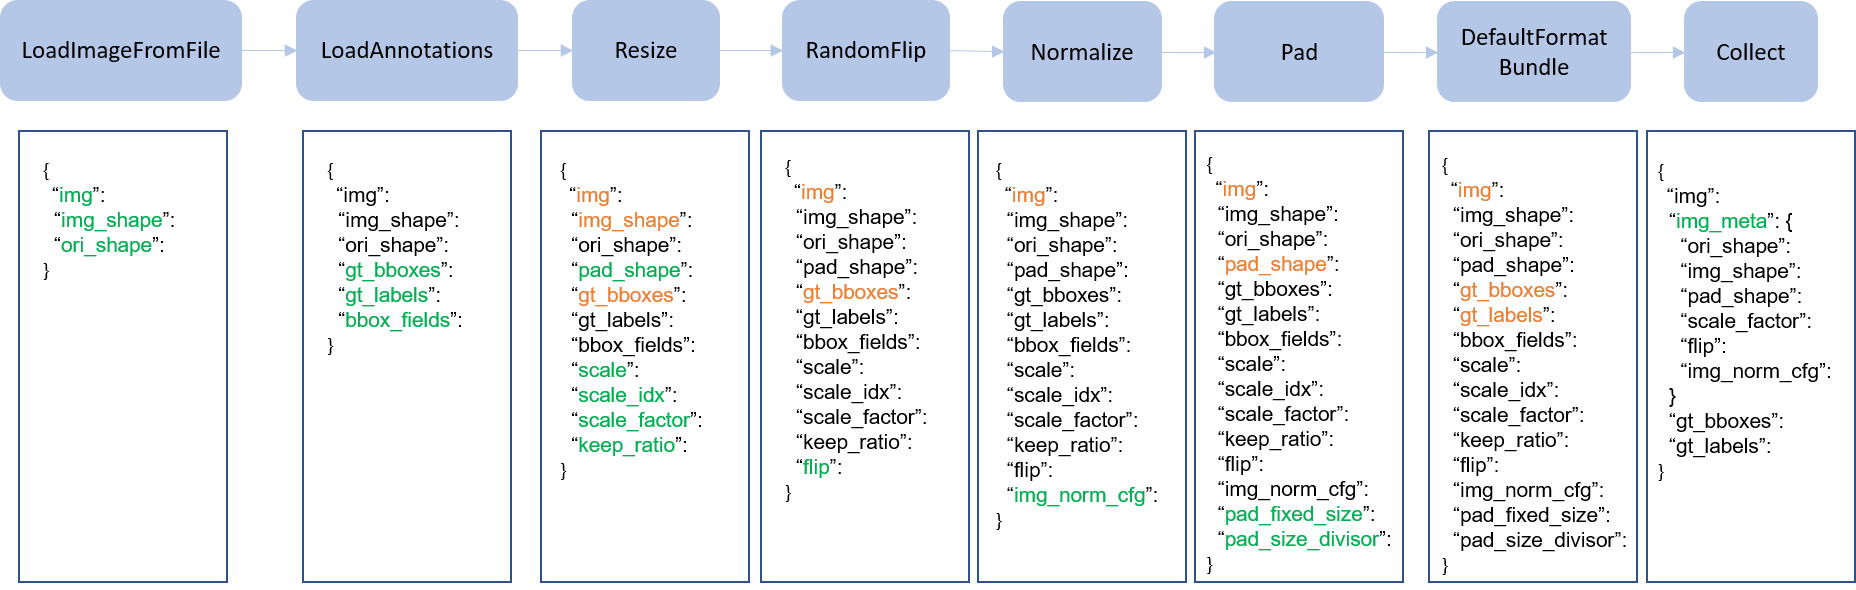
\includegraphics[width=9cm, height=3cm]{./pic/data_pipeline.png}
	\caption{ data pipeline }
\end{figure}

蓝色块为管道算子,一个算子为一个数据增强算法,从左到右,依次字典进,字典出。关于数据结构,可参考第二节数据处理。
这里绿色为算子作用后新增的keys,橙色为算子作用与已有keys的values后的更新标记。


\subsubsection{扩展pipelines}

\lstset{style=mystyle}
\begin{lstlisting}[language=Python]

# 1.实现新增强函数 my\_pipeline.py
# 和pytorch原始transforms中的增强方式一样,实现__call__方法的类即可
from mmdet.datasets import PIPELINES

@PIPELINES.register_module()
class MyTransform:

    def __call__(self, results):    # 输入的是mmdet设定的字典格式
        results['dummy'] = True
		return results
		
# 2. 导入新类.
from .my_pipeline import MyTransform

# 3. 配置文件调用

img_norm_cfg = dict(
    mean=[123.675, 116.28, 103.53], std=[58.395, 57.12, 57.375], to_rgb=True)
train_pipeline = [
    dict(type='LoadImageFromFile'),
    dict(type='LoadAnnotations', with_bbox=True),
    dict(type='Resize', img_scale=(1333, 800), keep_ratio=True),
    dict(type='RandomFlip', flip_ratio=0.5),
    dict(type='Normalize', **img_norm_cfg),
    dict(type='Pad', size_divisor=32),
    dict(type='MyTransform'),
    dict(type='DefaultFormatBundle'),
    dict(type='Collect', keys=['img', 'gt_bboxes', 'gt_labels']),
]
\end{lstlisting}


\subsection{增加新模块}
每一个组件都如上小节所给的三部曲,实现,导入,修改配置文件。每一步,mmdet中都有一些范例,分别看一下,就能实现改写。

\subsubsection{优化器}

一些模型可能需要对某部分参数做特殊优化处理,比如批归一化层的权重衰减。我们可以通过自定义优化器构造函数来进行细粒度参数调优。
\lstset{style=mystyle}
\begin{lstlisting}[language=Python]
from mmcv.utils import build_from_cfg

from mmdet.core.optimizer import OPTIMIZER_BUILDERS, OPTIMIZERS
from mmdet.utils import get_root_logger
from .cocktail_optimizer import CocktailOptimizer

@OPTIMIZER_BUILDERS.register_module
class CocktailOptimizerConstructor(object):

	def __init__(self, optimizer_cfg, paramwise_cfg=None):

	def __call__(self, model):

		return my_optimizer
	
\end{lstlisting}


\subsubsection{开发新组件}

\begin{itemize}
	\item backbone,参考MobilenetV2
	\item neck, 参考PAFPN
	\item head 参考Retinaface
	\item roi extractor, 参考 DCN ROIAlign
\end{itemize}

关于head相关组件,核心的点我认为在于数据的流向。基础变换层由forward函数得到变换的结果,怎么放到Loss中去,其中所涉及到的
数据细节操作,是比较关键的。mmdet中会在head模块中实现对应的loss函数,最终被汇集到检测模型的loss中去。分别调用各自的loss.step, 进行权重更新。

这里贴一个新增loss样例:
\lstset{style=mystyle}
\begin{lstlisting}[language=Python]

# 1.在 mmdet/models/losses/my_loss.py实现新的box回归函数
import torch
import torch.nn as nn

from ..builder import LOSSES
from .utils import weighted_loss

@weighted_loss    # 加权损失函数,可参考损失函数章节
def my_loss(pred, target):
	assert pred.size() == target.size() and target.numel() > 0
	loss = torch.abs(pred - target)
	return loss

@LOSSES.register_module
class MyLoss(nn.Module):

	def __init__(self, reduction='mean', loss_weight=1.0):
		super(MyLoss, self).__init__()
		self.reduction = reduction
		self.loss_weight = loss_weight

	def forward(self,
				pred,
				target,
				weight=None,
				avg_factor=None,
				reduction_override=None):
		assert reduction_override in (None, 'none', 'mean', 'sum')
		reduction = (
			reduction_override if reduction_override else self.reduction)
		loss_bbox = self.loss_weight * my_loss(
			pred, target, weight, reduction=reduction, avg_factor=avg_factor)

# 2.然后在mmdet/models/losses/__init__.py.中注册
from .my_loss import MyLoss, my_loss

# 3. 配置文件使用
loss_bbox=dict(type='MyLoss', loss_weight=1.0))

\end{lstlisting}

\subsection{1.x模型升级到2.0}

执行脚本 tools/upgrade\_model\_version.py。可能有小于 1\% 的绝对AP减小,具体可参见configs/legacy。

\subsection{2.0和1.x的不同之处}
主要有四点不同:坐标系,基础代码约定,训练超参数,模块设计。

\subsubsection{坐标系}
新坐标系与\href{https://github.com/facebookresearch/detectron2/}{detectron2}一致
treats the center of the most left-top pixel as (0, 0) rather than the left-top corner of that pixel. 
这句话的意思是将$bbox = [x1, y1, x1 + w - 1, y1 + h - 1]$改为$bbox = [x1, y1, x1 + w, y1 + h]$,这样更加
自然和精确(假设长或宽为1,则box退缩为点或线,这是有问题的),同理xyxy2xywh的长宽就不在+1了,生成的anhor的中心偏移也不在是0.5而是0了。
与此相关的改动有Box的编解码,与iou计算相关的nms,assinger。另外,现在的坐标为float,1.xx为int,与此相关的有ahchor与特征网格的中心
对齐问题,这对anchor-based的方法在性能上有一定影响(变好),ROIAlign也能更好的对齐,mask cropping and pasting更精准,
利用新的RoIAlign 去crop mask targets,会得到更好的结果,因为没有取整等误差了,而且在训练上也有~0.1s/iter的速度提升(少了取整操作)。

\subsubsection{Codebase Conventions}

\begin{itemize}
	\item 类别设定,1.x中0为背景,$[1, k]$为$k$类对象,2.0中$k$为背景,$[0, k-1]$ 为$k$类对象。
	\item bbox分配方案就低质量分配上得到了改进。支持了更多长宽尺度输入,以上均有微弱性能提升。
	\item 配置名称约定改动为 $[model]\_(model setting)\_[backbone]\_[neck]\_(no
	\newline
	rmsetting)\_(misc)\_(gpu x batch)\_[schedule]\_[dataset].py$,
\end{itemize}


\subsubsection{训练超参数}
一些训练参数的优化
\begin{itemize}
	\item nms后的rpn的proposals从2000改为1000,(nms\_post=1000, max\_
	num=1000),mask, bbox AP有~0.2\%的提升。
	\item Mask, Faster R-CNN框回归损失函数Smooth L1 改为L1带来~0.6\%的提升,Cascade R-CNN and HTC保持原样。
	\item RoIAlign layer 采样数设置为0,0.2\%提升
	\item 默认设置不在使用梯度截断,这样训练更快,但RepPoints保持是为了训练稳定以及更好的结果。
	\item 默认的warmup ratio 从$1/3$改为$0.001$,这样更平滑,同时也是因为去掉了梯度截断。
\end{itemize}


\subsection{版本变化补充}
2.0相对于1.x版本,从代码上主要有这些改变:
\begin{itemize}
	\item[1.] core内部做了一些改写,比如anchor中的tagret移走了,增加了分割数据结构,抽象了bbox的编解码,新增iou\_calculators,看起来evaluation中的bbox\_overlaps不是最优的。
	\item[2.] 数据类做了更彻底的分解,将1.x版本的loader中的sample分离成和pipeline同级别,data\_loader放到数据类中的builder,结构更清晰。
	\item[3.] models中anchor\_heads改为dense\_heads;bbox\_heads, mask\_heads等two stage 相关的合并到roi\_heads中(和2思想一致)
	\item[4.] 所有registry.py均合并到builder.py中,更为简洁。
	\item[5.] necks增加了pafpn, detectors增加了fsaf,core/mask
	\item[6.] 配置文件采用了组合继承的方式。
	\item[7.] 优化了训练,测试流程,速度提升明显,版本支持pytorch1.5,1.2以下均不在支持,定制化模块做了优化。
\end{itemize}


\end{document}